%    Signály a soustavy
% notes:
%~~~~~~~~~
% \label{tky:eq003}
% \label{tky:exam000}
% \label{tky:fig000}
%---------------------------------------------------------------------------------------------------
% Setting path to image 
\graphicspath{{../src/TKY/img/}}
  \makeatletter
    \@addtoreset{chapter}{part}
  \makeatother
%---------------------------------------------------------------------------------------------------
% file SAS.tex
%---------------------------------------------------------------------------------------------------
\lstset{ %
  language=Matlab,                       % choose the language of the code
  basicstyle=\footnotesize,              % the size of the fonts that are used for the code
  backgroundcolor=\color{White},         % choose the background color. You must add \usepackage{color}
  commentstyle=\color{help}\textit,
  keywordstyle=\color{keyword}\textbf,
  breaklines=true,                       % sets automatic line breaking
  breakatwhitespace=true,                % sets if automatic breaks should only happen at whitespace
  showspaces=false,                      % show spaces adding particular underscores
  showstringspaces=true,                 % underline spaces within strings
  showtabs=true,                         % show tabs within strings adding particular underscores
  frame=none,	                           % adds a frame around the code - none, single
  tabsize=8,                             % sets default tabsize to 8 spaces
  captionpos=b,                          % sets the caption-position to bottom
  numbers=left,                          % where to put the line-numbers -none, left, right
  numberstyle=\footnotesize,             % the size of the fonts that are used for the line-numbers
  stepnumber=1,                          % the step between two line-numbers. If it's 1 each line
                                         % will be numbered
  xleftmargin=3em,                       % adjust left margin
}
\iftoggle{DEBUG}{
%  DEBUG was on
% ~~~~~~~~~~~~~~~~~~~~~~~~~~~~~~~~~~~~~~~~~~~~~~~~
%========================= Kapitola: Měření teploty ================================================
  % !TeX spellcheck = cs_CZ
%============ Kapitola: Regulační technika =========================================================
\chapter{Regulační technika}\hypertarget{tky:regulace}
\minitoc
  \section{Kde se vzala, tu se vzala, zpětná vazba}
    Protože stojící automobil má aktuální rychlost menší než žádaných \SI{50}{\km\per\hour}, 
    sešlápneme pedál plynu a automobil začne zrychlovat, což pozorujeme na tachometru. V momentě, 
    kdy je aktuální rychlost větší než žádaná, uvolníme v souladu s radami od instruktora pedál 
    plynu a rychlost automobilu začne klesat, až bude opět menší než je žádaných 
    \SI{50}{\km\per\hour}. Takto budeme dokola sešlapávat a uvolňovat pedál plynu, až dosáhneme 
    žádané rychlosti. Jistě si umíme představit, že rychlost dosažení žádané rychlosti, závisí 
    nejen na vlastnostech samotného automobilu, ale také na našich řidičských dovednostech. V 
    případě opatrného řidiče, bude rozjezd pomalý a tak se rychlost bude blížit žádané pomalu. V 
    případě zbrklého řidiče, bude rozjezd velice razantní, což povede k rychlému překročení žádané 
    rychlosti. Následné neuvážené odlehčení plynového pedálu povede k prudkému poklesu rychlosti, 
    viz zelený průběh na obr. \ref{tky:fig_feedback005}. V obou případech se nelze hovořit o dobrém 
    stylu jízdy. V prvním případě se řidič rozjíždí příliš dlouho, na vozovce představuje překážku 
    a delší dobu zbytečně unikají splodiny do ovzduší. Ve druhém případě je motor při extrémních 
    otáčkách příliš hlučný, dochází k nekvalitnímu spalování a opět k úniku škodlivin do ovzduší. 
    Styl jízdy nepůsobí příliš uklidňujícím dojmem na ostatní řidiče a účastníky silničního provozu.

    \begin{figure}[ht!] % \ref{tky:fig_feedback005}
      \centering
      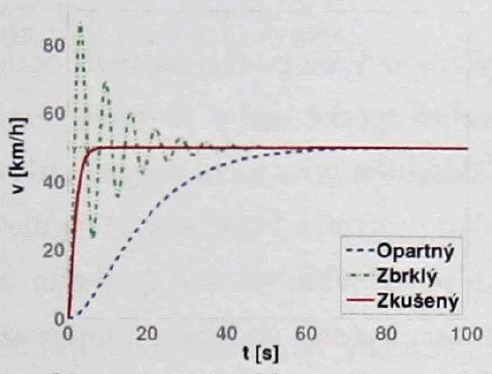
\includegraphics[width=0.7\linewidth]{Reg_smycka03.png}
      \caption{Rychlost automobilu \cite[s.~9]{Roubal2011}.}
      \label{tky:fig_feedback005}
    \end{figure}
    Pro kvalitní dosažení žádané hodnoty rychlosti je třeba znát \emph{dynamický model} automobilu. 
    Tedy nejen sešlápni pedál plynu, uvolni pedál plynu, což můžeme považovat za \emph{statický 
    model} (v čase neproměnný), ale právě popis jak rychle se automobil rozjíždí, když takovým a 
    takovým způsobem sešlápneme pedál plynu. V regulační technice budeme mít dynamický model 
    systému tvořený převážně diferenciálními (pohybovými) rovnicemi. Modelováním reálných 
    dynamických systémů se budeme zabývat v kapitole \ref{TKY:sec002}. Procesu získávání modelu 
    fyzikální reality říkáme \textbf{identifikace systému} a v našem příkladě s automobilem ji 
    vlastně provádíme tím, že se učíme jezdit. Na identifikaci dynamických systémů a její praktické 
    aspekty se zaměříme v kapitole \ref{TKY:sec003}.

    V momentě, kdy máme dynamický model systému, přichází další krok a to je vlastní \textbf{návrh 
    regulátoru}, neboli návrh algoritmu řízení. V momentě, kdy už řidič ví, jak automobil reaguje 
    na změny vstupu, může dosáhnout žádané výstupní veličiny mnohem lépe, viz obr. 
    \ref{tky:fig_feedback003}. Na rozdíl od řidiče, jenž má naučený regulátor ve své hlavě, v 
    regulační technice budeme využívat různé matematické metody. Možná nás nyní napadne, že model 
    automobilu není pouze závislost mezi pedálem plynu a rychlostí automobilu. Chování automobilu 
    ovlivňuje samozřejmě mnoho dalších okolností, jako je přilnavost pneumatik k povrchu vozovky, 
    vlhkost vozovky a podobně. V momentě, kdy například zaprší, může řidič se svým regulátorem v 
    zatáčce opustit vozovku, pokud jsme příliš agresivní, protože se reálný systém změnil, ale jeho 
    model tuto informaci nemá. Opět tedy musíme vzít v potaz nové faktory a provést identifikaci 
    znovu, a tím získat více informací o chování systému za těchto podmínek. Pak bude řidič schopen 
    jezdit bezpečně za sucha i za mokra a tak dále. V regulační technice je vždy přesnost modelu 
    zásadní otázkou. Na jedné straně požadujeme model systému co nejpřesnější, abychom byli schopni 
    navrhnout dobrý regulátor. Na druhé straně se pro příliš složitý model navrhuje regulátor 
    obtížněji. Proto vždy musíme zvolit jistý kompromis tak, aby v modelu byly zahrnuty všechny 
    podstatné vlastnosti systému.

    Tím ale regulace nekončí. Například cena paliva není již dnes zanedbatelná, a tak budeme třeba 
    chtít jezdit s minimální spotřebou. To znamená, že musíme zjistit závislost spotřeby paliva na 
    stylu jízdy. Poté musíme definovat nějaké kritérium kvality regulace obsahující tuto závislost 
    a podle něho navrhnout nový regulátor, který zajistí minimální spotřebu paliva.  Problémů v 
    oblasti řízení je samozřejmě mnohem a mnohem víc  (odhadování a filtrace, robustní řízení a 
    nelineární systémy). My však zde tento příklad ukončíme s konstatováním, že v regulační 
    technice jde především o tyto body:
    \begin{itemize}\addtolength{\itemsep}{-0.5\baselineskip}
      \item určení vstupů a výstupů systému,
      \item identifikace systému (určení chování systému na výstupech pro nějaké chování vstupů),
      \item návrh regulátoru pro zajištění požadovaných vlastností; testování regulátoru na 
            počítači; aplikace regulátoru na reálném systému; případně návrh v nějakém smyslu 
            optimálního regulátoru.
    \end{itemize}
    
  \section{Regulační smyčka a základní typy PID regulátorů}\label{TKY:sec001}
    Ve snaze řídit systémy rozeznáváme dva hlavní způsoby řízení:
      \begin{itemize}
        \item \textbf{přímovazební},
        \item \textbf{zpětnovazební}.
      \end{itemize}
    \textbf{Přímovazební řízení} (\emph{řízení v otevřené smyčce}), zvané také jako ovládání, má 
    jednodušší zapojení, ovšem jeho nevýhodou je nemožnost reagovat na poruchy či změny soustavy a 
    my se jím zde dále zabývat nebudeme. Naproti tomu \textbf{zpětnovazební řízení} (\emph{řízení v 
    uzavřené smyčce}), obecně označované jako \textbf{regulace}, porovnává \emph{výstup soustavy} 
    \(y(t)\) s \emph{požadovaným výstupem} \(w(t)\), a podle této informace generuje \emph{akční 
    zásah} \(u(t)\) do řízeného systému. Regulace nám tak dává mimo jiné možnost 
    \emph{stabilizovat} nestabilní soustavy.

    \begin{figure}[ht!] % \ref{tky:fig_feedback003}
      \centering
      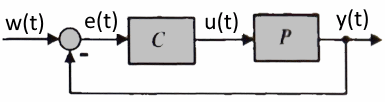
\includegraphics[width=0.8\linewidth]{Reg_smycka01.png}
      \caption{Regulační smyčka \cite[s.~215]{Roubal2011}.}
      \label{tky:fig_feedback003}
    \end{figure}
    V této kapitole se budeme věnovat regulaci, regulační smyčce a základním typů regulátorů. 
    Ukážeme si dvě základní zapojení regulačních smyček a zavedeme jednotné názvosloví, zejména 
    proto, že toto názvosloví není ustálené. Vysvětlíme si některé míry kvality řízení a ukážeme 
    názorně na příkladech vlastnosti základních \textbf{PID regulátorů}. Zvláštní pozornost bude 
    věnována filtraci derivační složky u tohoto regulátoru. Konkrétní způsoby návrhu regulátorů si 
    ukážeme v následujících kapitolách.
    
  
  \section{Modelování fyzikálních systémů}\label{TKY:sec002}
    Doposud jsme se v předešlých kapitolách zabývali různými nástroji, jak popisovat dynamické 
    chování systémů. Šlo spíše o teorii rozdělenou do kapitol bez větších souvislostí. V této kar 
    kapitole bychom chtěli ukázat použití těchto teoretických poznatků na konkrétních příkladech 
    fyzikálních systémů. Odvodíme zde několik matematických modelů fyzikálních systémů a připravíme 
    k těmto modelům simulinkové soubory s virtuální realitou pro Matlab (The Mathworks, 2009).
    
  \section{Identifikace systémů}\label{TKY:sec003}
    
%---------------------------------------------------------------------------------------------------
\printbibliography[title={Seznam literatury}, heading=subbibliography]
\addcontentsline{toc}{section}{Seznam literatury} 
}
{
% DEBUG was off
%======================= Kapitola: Základy technické kybernetiky ===================================
  % !TeX spellcheck = cs_CZ
%======================= Kapitola: Základy technické kybernetiky ===================================
\chapter{Základy technické kybernetiky}
\minitoc
  \section{Vznik a vývoj kybernetiky}
    Kybernetika je jedním z nejmladších vědních oborů a její vznik spadá do čtyřicátých let 
    dvacátého století. Vznik je úzce spjat s vývojem mnoha jiných vědních oborů jako matematická 
    logika, fyziologie, neurofyziologie a s rozvojem některých technických oborů jako je 
    elektronika, výpočetní technika, řídicí technika. Kybernetika není vědou, která by pouze 
    přebírala poznatky jiných věd. Ona hledá to, co jednotlivé vědní obory spojuje, postihuje 
    určité společné rysy různých vědních oborů a má snahu o jejich integraci. 

    \begin{figure}[ht!]
      \centering
      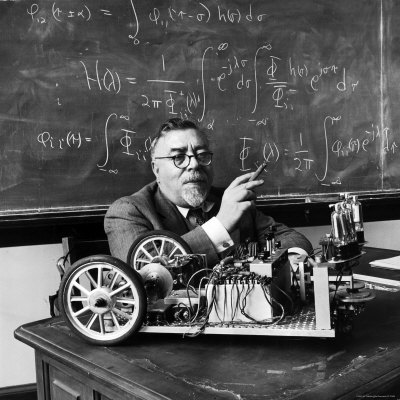
\includegraphics[width=0.8\linewidth]{Norbert_Wiener.jpg}
      \caption{Norbert Wiener (26. listopadu 1894 – 18. brezna 1964) byl americký matematik, který 
               je považován za zakladatele kybernetiky. }
      \label{tky:fig003}
    \end{figure}
  
    Historicky poskytlo impuls ke vzniku kybernetiky řešení problému řízeni palby protiletadlového 
    dělostřelectva za 2. světové války. Na tomto úkolu pracoval také americký matematik 
    \emph{Norbert Wiener}. Výsledkem matematického i konstrukčního úsilí bylo, že mířič - člověk 
    byl nahrazen přístrojem - zaměřovačem, který snímal údaje o současné poloze letadla, z ní 
    vypočítával polohu v budoucích okamžicích a servomechanismem se přenášela informace od 
    zaměřovače a počítače na kanóny. Norbert Wiener pak jako první zpracoval teorii 
    automatizovaných systémů řízeni pro účely protiletecké obrany. Tuto teorii zobecnil pro všechny 
    druhy technických, biologických a společenských systémů. Shrnul ji ve své proslulé knize 
    \emph{Kybernetika neboli řízení a sdělování v živých organismech a strojích}. Tato kniha vyšla 
    v roce \num{1948} a stala se světovým vědeckým bestsellerem. Svého autora proslavila jako 
    zakladatele kybernetiky.
    
    Řešení praktických (a bohužel vojenských) problémů použití elektronických počítačů k řízení 
    střel inspirovalo Wienera ke studiu řízení se zpětnou vazbou. Spolu s neurofyziologem 
    \emph{Arturem Rosenbluethem} hledali analogie k technickým zpětnovazebním systémům pro navádění 
    střel na pohyblivý cil. Takovou analogii nalezli u některých biologických systémů - konkrétně v 
    nervové soustavě živých organismů. Myšlenka zpětné vazby u živých a neživých systémů se stala 
    základem kybernetické koncepce vyložené v citované knize. Hledáni analogií mezi živým 
    organismem a strojem (případně také společnosti) znamená postihnout společné znaky zdánlivě 
    naprosto různorodých systémů. A tyto analogie pak vedou k používáni matematického a logického 
    aparátu i tam, kde to dosud nebylo možné.
    
    Nemůžeme ovšem nevidět všechny předcházející tendence a faktory v historii společnosti, které 
    vedly ke vzniku kybernetiky. Bylo by nesprávné tvrdit, že pouze Norbert Wiener a několik jeho 
    spolupracovníků vytvořilo kybernetiku. Její vznik byl pokračováním určité tendence, která se 
    projevovala již dávno předtím. Kybernetiku musíme chápat jako výsledek rozvoje materiálních sil 
    lidské společnosti a rozvoje vědeckého poznáváni světa.
    
    Název kybernetika pochází z řeckého slova \uv{kybernétés} neboli \uv{kormidelník}, \uv{člověk 
    řídící loď}. Objevuje se v dílech řeckých filosofů, např. v Platonově díle Dialogy; zde se 
    tímto termínem vyjadřuje \uv{umění řídit lodě a administrativně spravovat provincie}. V 
    novověku použil termín kybernetika A. M. Ampére v encyklopedii a to ve smyslu \uv{vědy o řízení 
    společnosti}. Termín se neujal a tak to byl až Wiener, který jím nazval nově vznikající vědní 
    obor. \cite[s.~6]{Svarc1986}.

    \subsection{Základní pojmy kybernetiky a její vymezení}
      Pro kybernetiku jsou charakteristická tři základní hlediska, z kterých nazírá na problémy a z 
      kterých dané problémy řeší. Jsou to      
      \begin{figure}[ht!]
        \centering
        % Set the overall layout of the tree
        \tikzstyle{level 1}=[level distance=5cm, sibling distance=1cm]
        
        % Define styles for bags and leafs
        \tikzstyle{bag} = [text width=14em, align=flush right]
        \tikzstyle{end} = [text width=10em, align=flush left]
        
        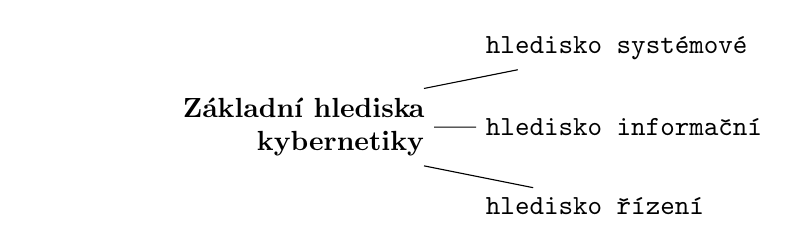
\begin{tikzpicture}[grow=right, sloped]
        \node[bag] {\textbf{Základní hlediska kybernetiky}}
            child {
                node[end] {\texttt{hledisko řízení}}
            }
            child {
                node[end] {\texttt{hledisko informační}}
            }
            child {
                node[end] {\texttt{hledisko systémové}}
            };
        \end{tikzpicture}
        \caption*{ }
      \end{figure}
      
      Tím se dostáváme k nejzákladnějších pojmů kybernetiky: \textbf{systém}. \textbf{informace} a 
      \textbf{řízení}, Z těchto hledisek se pak vyvinuly základní obory teoretické kybernetiky - 
      teorie systémů, teorie informace a \hyperlink{tky:regulace}{teorie řízení}.
      
      Jako příklad vysvětlující tato hlediska kybernetiky si zvolme automobil. Automobil je z 
      hlediska konstruktéra složité technické zařízení, sloužící k dopravě osob a nákladu, které je 
      vyrobeno z různých materiálů. Je sestaven z mnoha součásti, pohon je motorem spalovacím nebo 
      vznětovým, k provozu jsou nezbytné látky jako benzín, oleje, voda, ... .To vše je důležité a 
      podstatné z hlediska konstruktéra automobilu, ale ne z hlediska kybernetiky.
      
      Jaká jsou tedy hlediska kybernetiky? Kybernetika vidí v automobilu především tzv. 
      \textbf{dynamický systém}, jehož činnost je spojena s člověkem - řidičem a je ve vztahu k 
      okolnímu světu. Automobil uvažovaný jako systém se skládá ze dvou podsystémů (subsystémů). 
      Prvním z nich je vlastní vozidlo, druhým je člověk. Každý podsystém se pak skládá z 
      elementárních jednotek, vzájemně propojených, tzv. \emph{prvků systému}. Mezi prvky systému 
      existují různé vztahy. Ale nejenom mezi prvky nebo podsystémy existuji vztahy.

      \begin{wrapfigure}[11]{r}{6cm}   %\ref{tky:fig001} 
        \centering
        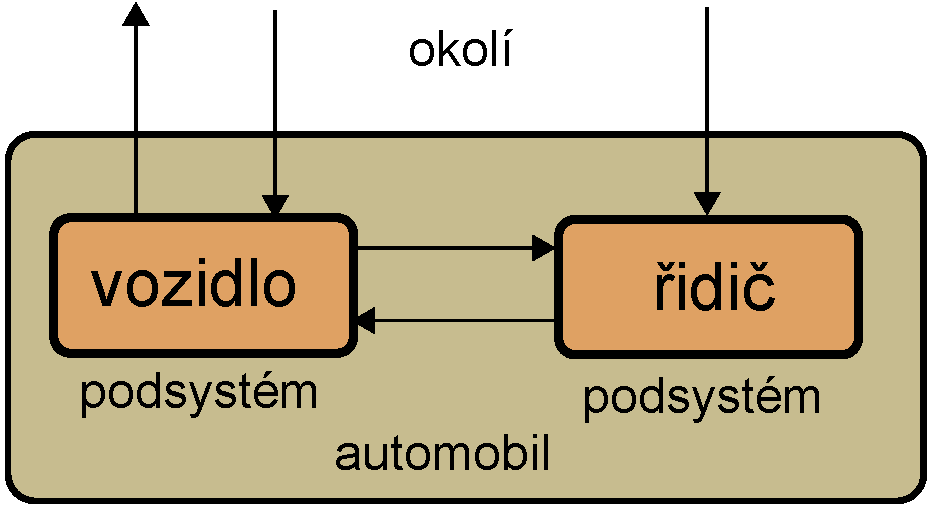
\includegraphics[width=0.9\linewidth]{tky_automobil.pdf}
        \caption{ }
        \label{tky:fig001} 
      \end{wrapfigure} 
      Automobil není izolovaným systémem a proto má také četné vztahy k okolí. K okolí \uv{systému 
      automobil} patří ty části okolního světa, které mají vliv na jeho činnost. Jsou to např. 
      vozovka, křižovatky, zatáčky, jiná vozidla, chodci, dopravní značky apod. Na všechny vlivy 
      okolí reaguje systém automobil určitým způsobem. Reakce systému na okolí se nazývá 
      \textbf{chováni systému}. Pokud sleduje kybernetika automobil tímto způsobem, jedná se o 
      \emph{systémové hledisko} kybernetiky  (obr. \ref{tky:fig001}). Předběžně si vymezme pojem 
      systém jako soubor prvků, mezi nimiž existuji nějaké funkční vztahy. Sledujeme-li vzájemné 
      působeni systému a jeho okolí, jde o druhé základní kybernetické hledisko. Poněvadž se toto 
      působeni realizuje výměnou informaci mezi systémem a okolím, mluvíme o \emph{informačním 
      hledisku}. Pod pojmem informace si představíme zprávu, která má pro některé ze zúčastněných 
      systémů určitý význam. Nositelem informace jsou tzv. \textbf{signály}.
      
      Doposud jsme uvažovali prostou výměnu informaci mezi dvěma systémy. Je-li ale informace 
      využívána přijímacím systémem pro další činnost, pro dosaženi určitého předem stanoveného 
      cíle, pak už se jedná o \emph{řízení}. Pojem řízení vymezíme jako \emph{proces výměny 
      informace mezi dvěma systémy}, který se uskutečňuje plánovitě pro dosažení určitého cíle. Při 
      řízení se uplatňuje informační působení řídicího systému na řízený systém. Tím se dostáváme k 
      třetímu kybernetickému hledisku a to je \emph{hledisko řízení}. Zdůrazněme, že toto hledisko 
      provádí pouze informační bilancování a nikoliv látkové nebo energetické.
      
      Vraťme se k našemu automobilu. Systém automobil má dva podsystémy vozidlo a řidiče. Mezi nimi 
      probíhá informační výměna, jejíž cílem je pohyb automobilu po stanovené dráze, např. v přímém 
      směru. Řidič reaguje na nerovnosti vozovky nebo na boční vítr, které vychyluji vozidlo z 
      přímého směru tím, že pootáčí volantem. Řidič je tedy řídícím systémem a vozidlo řízeným 
      systémem a výměna informací probíhá za účelem udrženi pohybu vozidla v přímém směru - jedná 
      se o \textbf{proces řízení}.
      
      Všimněme si momentu, že řidič otáčí volantem na základě toho, jaký účinek vyvolalo předchozí 
      pootočení. Neustále sleduje směr vozidla a vyrovnává odchylky od přímého daného směru. Takový 
      způsob řízení označujeme v kybernetice jako \textbf{řízení se zpětnou vazbou} neboli 
      \textbf{regulace}. Systémy se zpětnou vazbou se tedy nazývají \textbf{regulační systémy}. 
      Systém automobil (řidič + vozidlo) můžeme pokládat za regulační systém, který je regulován na 
      přímý směr jízdy.
      
      Poněvadž systémy řízení se zpětnou vazbou, tedy regulační systémy, jsou pro kybernetiku 
      charakteristické, nazýváme třetí kybernetické hledisko také \emph{hlediskem regulačním}. 
      Samozřejmě existuje rovněž \textbf{řízení bez zpětné vazby}; v tom případě se mluví jen o 
      \textbf{systémech řízení} nebo o \textbf{systémech ovládání}.
      
      Řízení jako vzájemná interakce mezi systémy nebo mezi systémem a okolím probíhá vždy v 
      určitém pořadí činnosti některého ze systémů. obvykle řídicího. Soubor pravidel, podle něhož 
      řídící systém vykonává sled činností za účelem řízení, se nazývá \textbf{algoritmus}. Obecně 
      je \emph{algoritmus soubor pravidel, podle něhož probíhá řízení}.
      
      U zvoleného příkladu s automobilem bychom mohli například sestavit algoritmus spouštění 
      motoru, algoritmus vyjíždění automobilu, algoritmus předjíždění, atd. Algoritmy jsou objektem 
      zkoumání jednoho z oborů teoretické kybernetiky - \emph{teorie algoritmů}.
      
      Pe předběžném objasnění základních hledisek kybernetiky a základních pojmů kybernetiky je 
      možné se pokusit vyložit, ce vlastně kybernetika je a čím se zabývá. Jednotlivý autoři, kteří 
      se pokoušejí podat definici kybernetiky, protěžují více nebo méně některé ze tří základních 
      kybernetických hledisek (hledisko systémové, hledisko informační, hledisko řízení). Většina 
      starších definic kybernetiky vychází z klasické definice jejího uznávaného zakladatele 
      Norberta Wienera, který ji definoval jako \uv{vědu o řízení a sdělování v živých organismech 
      a strojích}. Tato definice, která je nerozlučně spjata s jejím vznikem, protěžuje hledisko 
      informační a hledisko řízení. Jejím nedostatkem je, že ještě nedoceňuje systémový přístup, 
      systémové hledisko při řešení problémů. Dále jako objekty zkoumání (tedy systémy) zahrnuje 
      pouze živé organismy a stroje. Nezahrnuje tedy další důležité objekty zkoumané dnešní 
      kybernetikou jako jsou objekty společenské a ekonomické a neuvažuje systémy matematické, 
      lingvistické a další a z technických systémů dnes tak různorodých se omezuje jen na stroje. 
      Ani informační hledisko této definice není úplné, protože se omezuje pouze na přenos 
      informaci a neuvažuje dnes tak důležité procesy uchování a zpracováni informace.
      
      Podobnými nedostatky se vyznačovaly definice kybernetiky dalších autorů. Byl to vždy 
      jednostranný přístup a neúplnost jednotlivých hledisek. Proto nelze žádnou z definic 
      akceptovat s definitivní platností.
      
      Nebudeme se tedy snažit za každou cenu zformulovat vyčerpávající definici, ale uveďme si 
      charakteristické rysy kybernetiky jako vědy.
      
      Kybernetika se zabývá různými rozdílnými problémy, které však byly většinou známy a zkoumány 
      před vznikem kybernetiky, např. krevní oběh, podmíněný reflex, radiolokace, konstrukce 
      počítačů, řízení různých technických zařízení, kódování atd. Kybernetika vnáší do těchto 
      problémů nový pohled, neboť si všímá toho, že na určitém stupni organizace a vývoje systémů 
      vzniká nový proces řízení. Tento proces se projevuje výměnou informací v systémech, kterým se 
      chování systémů zaměřuje k určitému cíli.
      
    \subsection{Rozdělení kybernetiky}
      Z praktického hlediska můžeme kybernetiku rozdělit podle přístupu a aplikací:
      \begin{itemize}\addtolength{\itemsep}{-0.5\baselineskip}
        \item \textbf{teoretická kybernetika},
        \item \textbf{aplikovaná kybernetika}.
      \end{itemize}

      \emph{Teoretická kybernetika} studuje především obecné vlastnosti a chování systémů. Zabývá 
      se obecným popisem vlastností a chování systémů. Z tohoto pohledu zahrnuje teoretická 
      kybernetika \emph{teorii systémů} a \emph{teoretickou informatiku}.
      
      \emph{Aplikovaná kybernetika} představuje použití kybernetického přístupu při analýze, 
      modelování a simulaci a návrhu systémů, dále aplikuje poznatky kybernetiky do dalších 
      oblastí. Aplikovaná kybernetika zasahuje do mnohých oblastí lidské činnosti - zahrnuje totiž 
      mj. následující obory:
      
      \begin{itemize}\addtolength{\itemsep}{-0.1\baselineskip}
        \item \textbf{Teoretická kybernetika}
              \begin{itemize}\addtolength{\itemsep}{-0.1\baselineskip}
                \item \emph{Dynamické systémy}: zpětná vazba, stavový popis, stochastické systémy,
                      řízení, aj.
                \item \emph{Přenos informace}: informační entropie, kapacita komunikačního kanálu, 
                      aj. 
                \item \emph{Umělá inteligence}: strojové vnímání a učení, multi-agentní systémy, 
                      robotika, modelování neuronových sítí, konekcionismus, vazba člověk-stroj, ...
                \item \emph{Teorie rozhodování}, her, teorie složitosti, chaotické systémy, aj.
              \end{itemize}
        \item \textbf{Informatika}
        \item \textbf{Biokybernetika}
        \item \textbf{...}
      \end{itemize}
      
  \section{Teorie systémů}
     Teorie systémů je jedna ze základních disciplin teoretické kybernetiky. Na druhé straně je ale 
     teorie systémů součásti tzv. \emph{obecné teorie systémů}, jejíž principy rozpracoval americký 
     biolog Ludwig von Bertalanffy. Pokusme se o vymezení vztahu mezi kybernetikou a teorií systémů.
     \cite[s.~11]{Svarc1986}.
     
     Obecná teorie systémů studuje systémy libovolné povahy, přičemž se zajímá o charakter prvků 
     systému, charakter vazeb mezi prvky a chováni systému. Důležitým pojmem je zde \textbf{vazba 
     mezi prvky} a pojem \textbf{chování systémů}. Zatímco obecná teorie systémů se zajímá o 
     libovolný druh vazeb mezi prvky a libovolné chování systémů, kybernetiku zajímá specifický 
     druh vazeb a specifické chování. Kybernetika studuje pouze ty vazby, které jsou realizovány 
     přenosem informace a chování, které lze zahrnout pod \textbf{pojmem řízení}. A to je náplni 
     teorie systémů jako discipliny teoretické kybernetiky.
     
     \textbf{Přenos informace} a \textbf{řízení} nejsou od sebe \emph{oddělitelné}. Aspoň tak, že 
     není možné řízení bez přenosu informace. Je však už sporné, je-li každý přenos informace již 
     řízením. Můžeme říci, že systémy mezi nimiž probíhá proces řízení musí mít určitou specifickou 
     strukturu a musí být mezi nimi zajištěn přenos informace. Pokud existuje pouhá výměna 
     informací mezi systémy, mluvíme o \textbf{informačních systémech}.
     
     \emph{Obecnou teorii systémů} tedy \emph{nemůžeme} zahrnout do kybernetiky; s kybernetikou má 
     společnou jen určitou část, která je zaměřena na studium systémů z hlediska informačních 
     vazeb. Hlavním úkolem obecné teorie systémů je postihnout a vyjádřit exaktním způsobem 
     vlastnosti a vztahy ve složité a dynamické (v čase se měnící) \emph{objektivní realitě} tak, 
     aby se neztratila její komplikovaná struktura a složitost. Jestliže dříve byl nějaký přírodní 
     nebo společenský jev pokládán za vysvětlený, když se nalezla jeho příčina, pak při systémovém 
     přístupu musí bý nalezena struktura a dynamika každého objektu, který se na daném jevu podílí.
     
     \subsection{Charakteristika základních pojmů z teorie systémů}
       Pro práci se složitými a rozsáhlými objekty, jako jsou například řízení výrobních a
       technologických procesů, je nutný \textbf{systémový přístup}. Například technologický proces
       exploatace uhlí na hlubinných nebo povrchových dolech, je charakterizován různorodostí
       pracovních činností, na něž působí celá řada vlivů. Komplexně jde o mnoha rozměrný
       dynamický celek, který se neustále mění v čase a v prostoru.
       
       \emph{Systémový přístup spočívá v tom, že jevy vyskytující se při řešení vzniklých problémů, 
       jsou chápany komplexně, se všemi souvislostmi ve svém dynamickém vývoji.}
       
       V souvislosti se systémovým přístupem je nejdůležitějším pojmem \textbf{systém}. Jestliže 
       chceme v dalším uvést základní pojmy teorie systémů, musíme nejdříve tento pojem vysvětlit. 
       Předběžně jsme ho vymezili jako \emph{soubor prvků, mezi nimiž existuji nějaké funkční 
       vztahy a který má jako celek vztah ke svému okolí}. Jinými slovy: \emph{Stanovíme- li 
       vztahy, mezi na sebe navzájem působících objektů materiální, ale i nemateriální povahy, je na
       objektivní realitě vytvořen systém.} Jiní autoři podávají tyto definice:
       \begin{itemize}\addtolength{\itemsep}{-0.5\baselineskip}
         \item Bertalanffy (1956): Systém je komplex prvků nacházejících se ve vzájemné interakci.
         \item Hall - Fagen (1966): Systém je souhrn prvků spolu se vztahy mezi prvky a mezi jejich 
               vlastnostmi.
       \end{itemize}

       \begin{definition}
        \textbf{Systém} je definován jako účelově uspořádaná množina prvků a množina vazeb mezi 
        nimi, s dynamickým chováním, které společně určují vlastnosti celku.
        \begin{equation}
          \mathscr{S} = \{S,R \},
        \end{equation}
        kde
        \begin{description}[leftmargin=5em,style=nextline]
          \item[\hspace{2em}\(S \ldots\)] \emph{množina všech prvků},
          \item[\hspace{2em}\(R \ldots\)] \emph{množina relací mezi prvky, reprezentující vzájmené 
                                         funkční vztahy jednotlivých prvků a vztah systému k okolí.}
        \end{description}
       \end{definition}
       
       V rámci dekompozice systému lze vyčlenit \textbf{podsystém}. Podsystém je podmnožina
       systémových prvků a vazeb, která je z nějakého důvodu vyčleněna ze systému a je chápána
       jako nový systém nebo jako prvek.
       
       \begin{definition}
        \textbf{Prvek} je část systému, který tvoří na dané rozlišovací úrovni dále nedělitelný 
        celek, jehož strukturu nechceme, nebo již nemůžeme v rámci analýzy rozlišit.
       \end{definition}
       
       \begin{note}
         \textbf{Rozlišovací úrovní} se označuje stupeň podrobnosti zkoumání systému. Změnou        
         rozlišovací úrovně se může dřívější prvek systému stát podsystémem, popřípadě i systémem a 
         naopak. Dekompozicí systému na jednodušší prvky, se zvyšuje rozlišovací úroveň.
       \end{note}
       
     \subsection{Klasifikace systémů}
       Někdy rozlišujeme pojem \textbf{statický} a \textbf{dynamický systém}, ale spíš známe pouze 
       systémy dynamické. Statický systém je totiž v čase konstantní, neměnný. Mezi statické 
       systémy můžeme někdy zařadit i systémy, u nichž se vlastnosti prvků mění velmi pomalu. V 
       přírodě se statické systémy prakticky nevyskytují, spíše se jedná o systémy s pomalou změnou 
       vlastností na čase. Naproti tomu dynamický systém je takový systém, u kterého existuje 
       alespoň jedna proměnná závislá na čase. Většina systémů je dynamických. V dalším textu jsou 
       proto popsány především \textbf{dynamické systémy a řídicí (regulační) systémy se zpětnou 
       vazbou}.
       
       Dynamické vlastnosti lineárních systémů lze popsat lineárními diferenciálními rovnicemi s 
       konstantními koeficienty a operátorovými přenosy. Dynamické vlastnosti nelineárních systémů 
       lze popsat nelineárními diferenciálními rovnicemi.
       
       Existují dvě možnosti studia dynamického systému. Prvním způsobem je zkoumání \emph{vnitřní 
       struktury systému}, tzn. vnitřní závislosti prvků a dále nás zajímají, jaké vnitřní změny 
       vznikají v systému při působení vnějších vlivů. To je podstatou \textbf{vnitřního popisu 
       dynamického systému}.
       
       Druhým způsobem je pojímání systému jako celek a studování pouze otázky, jaké výsledné 
       reakce systému vyvolávají vnější vlivy. Tomuto druhému způsobu se budeme věnovat při 
       \textbf{vnějším popisu dynamických systémů}.
     
     
  \section{Teorie informace}
    \textbf{Informace} jako stěžejní pojem kybernetiky, je pojem značně široký a hodně diskutovaný. 
    Je používán v celé řadě definic vymezujících předmět kybernetiky jako vědy, přičemž informační 
    hledisko považují někteří autoři za nejdůležitější.
      
    Přesná definice pojmu informace neexistuje. Obecně se tento pojem používá volně, v intuitivním 
    chápaní se vztahuje k pojmům jako zpráva, údaj, poznatek apod. Z hlediska kybernetiky je toto 
    chápáni příliš zúženo, neboť kybernetika sleduje přenos informace mezi dvěma nebo více systémy 
    s tím, že cílem přenosu může být řízení chování některého ze systému. Kybernetika říká, že 
    informace je jakékoliv sdělení, kterého lze reálně (právě nyní) nebe potenciálně (v budoucnu 
    při vhodné příležitosti) použit k řízeni systému.
    
    Pojem informace je \emph{pojmem abstraktním} a jako takový má \emph{nehmotnou povahy}. 
    Současně však informace má smysl jen ve spojení s hmotou a to jak z hlediska přenosu, tak z 
    hlediska obsahu (i abstraktní představy jsou spjaty s existenci hmoty).
    
    Informace (sděleni) má
    \begin{itemize}\addtolength{\itemsep}{-0.4\baselineskip}
      \item \textbf{formu},
      \item \textbf{obsah},
      \item \textbf{význam}.
    \end{itemize}
    \textbf{Forma} informace neboli sdělení musí být přístupná systémům, mezi nimiž dochází k 
    výměně informaci a je důležitá pro proces přenosu informace. Pro proces řízení systémů je 
    podstatný \textbf{obsah a význam informace} (sdělení). \textbf{Sdělení} je \emph{informační, 
    sémantický a pragmatický obsah}. \textbf{Informační obsah} vyjadřuje kvantitativní míru 
    informace v dále definované jednotce \textbf{bit}. Používáme pro něj termín míra či množství 
    informace. \textbf{Sémantický obsah} vyjadřuje významovou stránku znaků při jazykové komunikaci 
    a nedá se měřit (\emph{sémantika} - nauka o významu slov). \textbf{Pragmatický obsah} určuje 
    významnost sdělení a prioritu jednotlivých zpráv pro příjemce.
    
    Každá forma hmoty, která nese informaci se nazývá \textbf{zpráva}. Zpráva je hmotným nositelem 
    informace. Zpráva je způsob vyjádření informace textem, obrazem, řečí, posloupností znaků atd. 
    Zpráva může být tedy např. číslo (posloupnost číslic), abecední text (posloupnost písmen), 
    spouštěcí signál (posloupnost napěťových úrovní). Pojmy informace a zpráva nelze zaměňovat. 
    Informace jo pojem abstraktní, zpráva jo konkrétní materiální formou informace, bez níž by 
    informace neměla smysl a nemohla by být přenášena a působit na systémy, kterým je určena. Pojem 
    zpráva bývá někdy nahrazován užším pojmem \textbf{signál}. Signál je fyzikální realizace zprávy 
    ve formě elektrického proudu resp. elektromagnetických vln.
      
    Sledujeme-li blíže jakoukoliv dostatečně dlouhou zprávu, pak zjistíme, že je vždy vytvářena z 
    posloupnosti nějakých základních elementů - \textbf{prvků}. Možný počet odlišných prvků, ze 
    kterých je taková zpráva vytvářena, může být bud \emph{konečný} nebo \emph{nekonečný}. Tak 
    např. psaná zpráva ve formě českého textu je posloupností různých kombinací písmen české 
    abecedy. Možný počet různých písmen - prvků je konečný a je dán počtem písmen české abecedy.
      
    Základní prvky, ze kterých je vytvářena zpráva, bývají obecně nazývány \textbf{písmena} a celý 
    \emph{soubor} všech \emph{možných prvků} bývá nazýván \textbf{abecedou zdroje}. Zpráva je pak 
    vytvářena výběrem prvků z abecedy zdroje a jejich sestavou v posloupnost prvků. Přitom 
    libovolný prvek abecedy se může ve zprávě libovolně opakovat. Abychom mohli odlišovat prvky 
    abecedy od prvků, z nichž je sestavena konkrétní realizace zprávy, budeme libovolný prvek 
    realizace zprávy nazývat \textbf{symbol}. Nechť má abeceda zdroje celkem \(s\) možných různých 
    prvků. Nechť je délka zprávy, tj. počet symbolů, z nichž je složena realizace zprávy, dána 
    počtem \(L\) symbolů. Celkový možný počet \(L\) různých realizaci zpráv délky \(n\), které 
    mohou být produkovány zdrojem s abecedou o \(s\) prvcích a které se budou lišit nejméně v 
    jednom symbolu, je
    \begin{equation}\label{tky:eq0001}
      L = s^n
    \end{equation}
    (počet všech možných \emph{variací n symbolů s opakováním}, které lze vytvořit z \(s\) prvků).
    
    Má-li abeceda zdroje \emph{konečný počet} \(s\) možných prvků, pak takový zdroj nazýváme 
    zdrojem \textbf{diskrétních zpráv} (diskrétní zdroj). Má-li abeceda zdroje \emph{nekonečný 
    počet prvků}, pak ho nazýváme zdrojem \textbf{spojitých zpráv} (spojitý zdroj).
    
    \begin{example}
      Kolik zpráv o délce \num{10} symbolů můžeme vytvořit z abecedy o \num{2} písmenech?
      \newline
      Řešení: Počet realizaci \(L\) zpráv je dán vztahem (\ref{tky:eq0001})
      \begin{equation*}
        L = s^n = 2^{10} = 1024
      \end{equation*}      
    \end{example}
      
    \subsection{Přenos zpráv}
      Zprávu lze přenést buď \emph{přímo}, přenesením nosného média (pergamen, magnetická páska, 
      optický disk), anebo \emph{nepřímým} způsobem prostřednictvím \emph{signálu}, který je 
      realizací zprávy ve formě změn některé fyzikální veličiny, nejčastěji elektrického proudu.
      
      Při nepřímém způsobu \textbf{zdroj informace} generuje prostřednictvím \textbf{kodéru} 
      (kódovacího zařízeni) signály, které se přenáší \textbf{kanálem}. Kanál je vlastně cesta, 
      která přenáší změny dané fyzikální veličiny, aby mohla být zpráva přenesena z jednoho místa 
      na druhé. Je tvořený prostředím, kterým se přenáší signál. Může to být např. telefonní 
      vedeni, trubka pro přenos tlakového signálu, akustické nebe elektromagnetické vlnění.
      
      Na výstupu kanálu je signál přijímán \textbf{příjemcem informace} (Člověk nebe zařízeni). 
      Zná-li příjemce zákon, podle kterého byla provedena transformace zprávy na vstupu kanálu, pak 
      může určit zprávu obsaženou v přijatém signálu. To provede tzv. \emph{dekódováním} v zařízeni 
      zvaném \textbf{dekodér}. Souhrn všech uvedených objektů vytváří \textbf{sdělovací soustavu}.

      \begin{figure}[ht!]
        \centering
        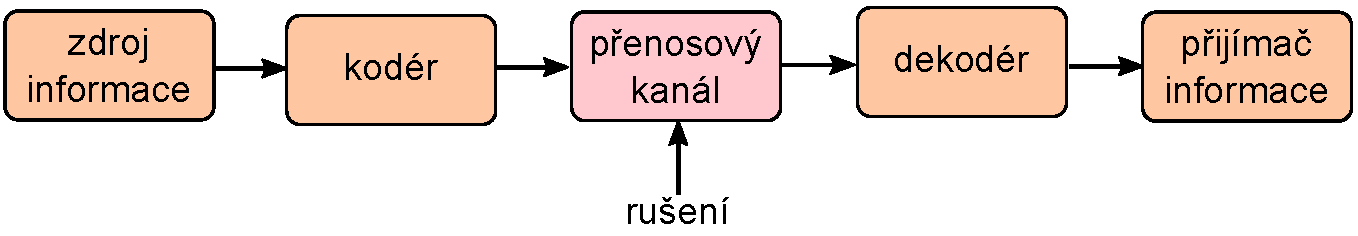
\includegraphics[width=0.9\linewidth]{tky_prenosovy_kanal.pdf}
        \caption{Nepřímý penos zprávy skrz přenosový kanál}
        \label{tky:fig002}
      \end{figure}

      Přenos signálu se může uskutečňovat v prvotní formě anebo v zprostředkované nepřímé formě, 
      kdy se pro přenos signálů používají pomocné tzv. \textbf{nosné signály}.
      
      Příkladem přenosu signálu v prvotní formě je přenos spojitých údajů o teplotě     
      prostřednictvím elektrického napětí ve vedení, přímo úměrné teplotě. 
      
      Při přenosu signálu v nepřímé formě se upravuje nosný signál tak, aby změny některého z jeho 
      parametrů zobrazovaly přenášenou zprávu. Tuto operaci vůči nosnému signálu nazýváme 
      \textbf{modulací}.
      
      
%---------------------------------------------------------------------------------------------------
\printbibliography[title={Seznam literatury}, heading=subbibliography]
\addcontentsline{toc}{section}{Seznam literatury} 
%======================= Kapitola: Číslicové signály - posloupnosti ================================
  % !TeX spellcheck = cs_CZ
%============ Kapitola: Číslicové signály - posloupnosti ===========================================
\chapter{Číslicové signály - posloupnosti}
\minitoc

  Číslicové signály (matematicky posloupnosti čísel) \cite{Sovka} jsou v literatuře
  oz\-na\-čo\-vá\-ny symboly $x_n, x(n)$, nebo $x[nT]$, kde $n$ je celé číslo a označuje pořadí
  prvku v posloupnosti\footnote{Takto zavedené označení je nejednoznačné, neboť nerozlišuje mezi
  celou posloupností a jejím jediným prvkem. Posloupnost by měla být správně označena např.
  symbolem $\{x[n]\}$, zatímco symbol $x[n]$ by měl být vyhrazen pro její jeden prvek. Nicméně
  uvedené značení je všeobecně používáno.} Poslední uvedený symbol $x[nT]$ zdůrazňuje souvislost
  číslicového signálu se signálem spojitým v čase(analogovým signálem), ze kterého vznikl
  vzorkováním a kvantováním. Symbol $T$ označuje použitý \emph{vzorkovací krok}. Jeho převrácená
  hodnota je rovna \emph{vzorkovací frekvenci} $f_s=\frac{1}{T}$.

  \section{Základní typy posloupností}
    \begin{itemize}
      \item \textbf{Jednotkový impuls}
            \begin{equation}\label{SAS:eq_jednotkovy_imp}
              \delta[n]=
              \begin{cases} 
                 1, &  n = 0, \\
                 0, &  n \neq 0,
              \end{cases}
            \end{equation}
      \item \textbf{Jednotkový skok}
            \begin{equation}\label{SAS:eq_jednotkovy_skok}
              u[n]=
              \begin{cases} 
                 1, &  n \geq 0, \\
                 0, &  n < 0,
              \end{cases}
            \end{equation}
      \item \textbf{Reálná exponenciální posloupnost}
            \begin{equation}\label{SAS:eq_exp}
              x[n] = A\alpha^n, n\geq0,
            \end{equation}
      \item \textbf{Chirp signál}
            \begin{equation}\label{SAS:eq_chirp}
              x[n] = sin\left(\frac{\pi f_{max}n^2}{(N-1)f_s}\right),
            \end{equation}
            kde $f_{max}$ je maximální požadovaný kmitočet, který musí být menší než polovina
            vzorkovacího kmitočtu $f_{max}<\frac{f_s}{2}$ a $N$ je celkový počet vzorků.
      \item \textbf{Pseudonáhodná posloupnost} je posloupnost, která nahrazuje ideální bílý šum.
            Tuto posloupnost lze generovat různými algoritmy, které zaručují velmi dlouhou 
            periodicitu generované posloupnosti. Má-li tato posloupnost aproximovat bílý šum, musí 
            co nejlépe splňovat požadavek nekorelovanosti sousedních vzorků (tedy konstantní 
            spektrální výkonové hustoty) a nulové střední hodnoty. Často je požadován i jednotkový 
            rozptyl.
            \begin{figure}[ht!]
             \centering
             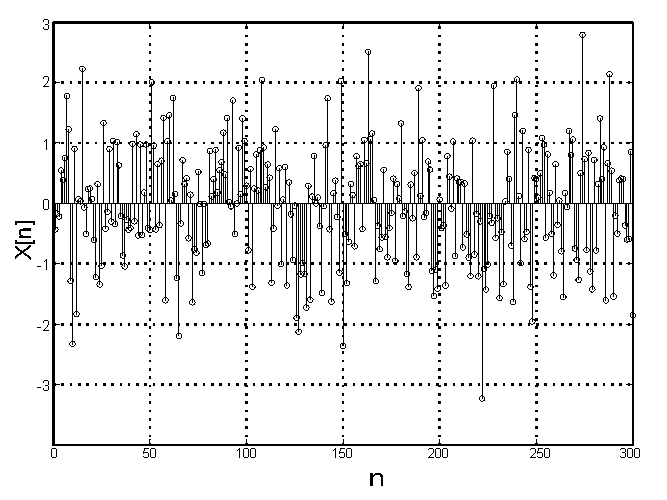
\includegraphics[width=0.8\linewidth]{randn_posloupnost.pdf}
             \caption[Příklad pseudonáhodné posloupnosti]{Příklad pseudonáhodné posloupnosti
                      generované pomocí funkce \texttt{randn(1, 300)} v MATLABu}
             \label{SAS:fig_randn}
         \end{figure}
    \end{itemize}
  
  \newpage
  \section{Generování jednoduchých signálů a jejich zobrazení v MATLABu}
    %---------------------------------------------------------------
    % !TeX spellcheck = cs_CZ
\begin{example}
  Generujte signál s lineárně rostoucím kmitočtem "\texttt{chirp signál}", maximální kmitočet
  $f_{max} = 20 Hz$, amplituda $A = 1$, vzorkovaný kmitočtem $f_s = 64 Hz$.

    {\centering
     \begin{tabular}{c}
         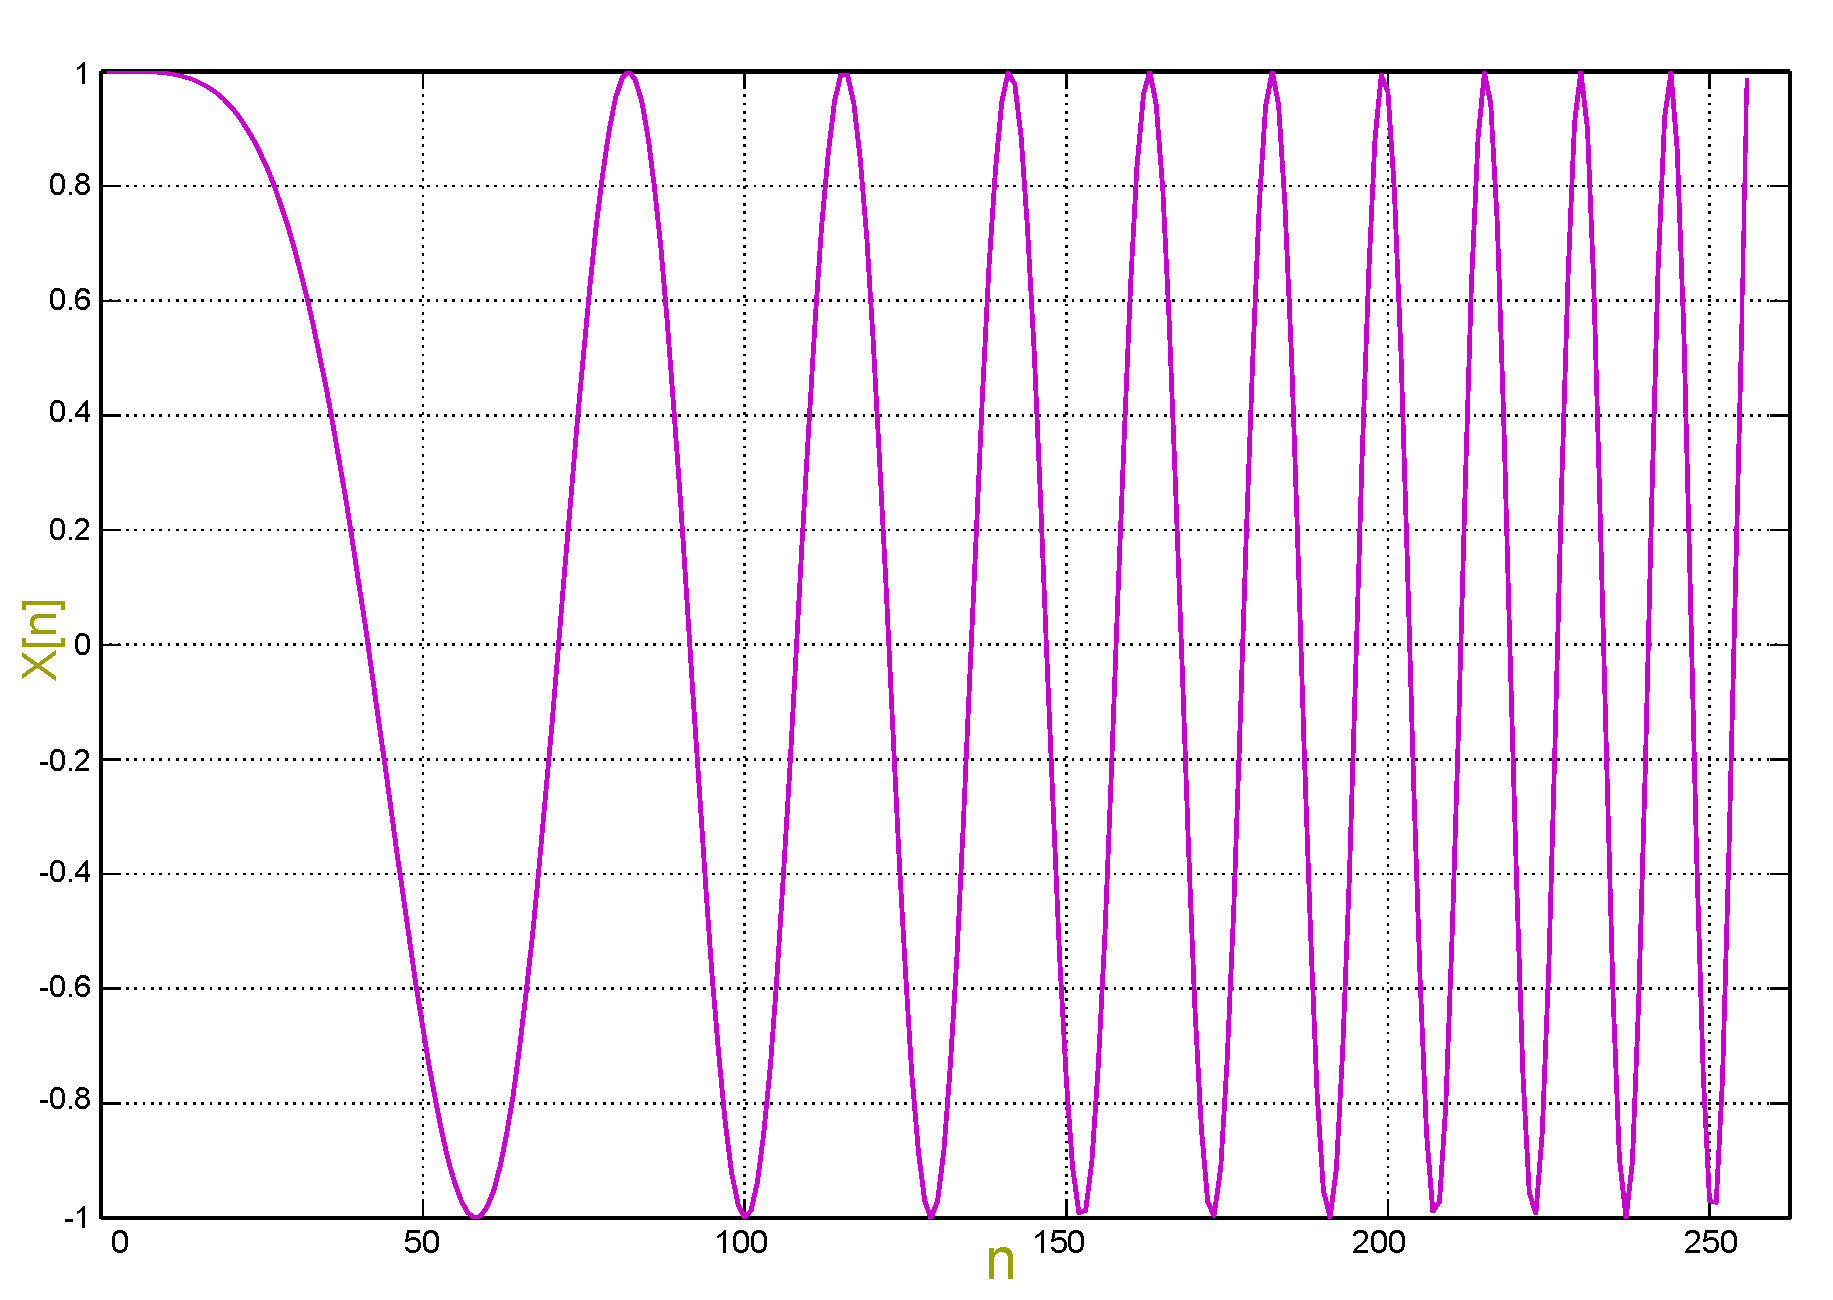
\includegraphics[width=0.8\linewidth]{Chirp_signal_plot.pdf}  \\
         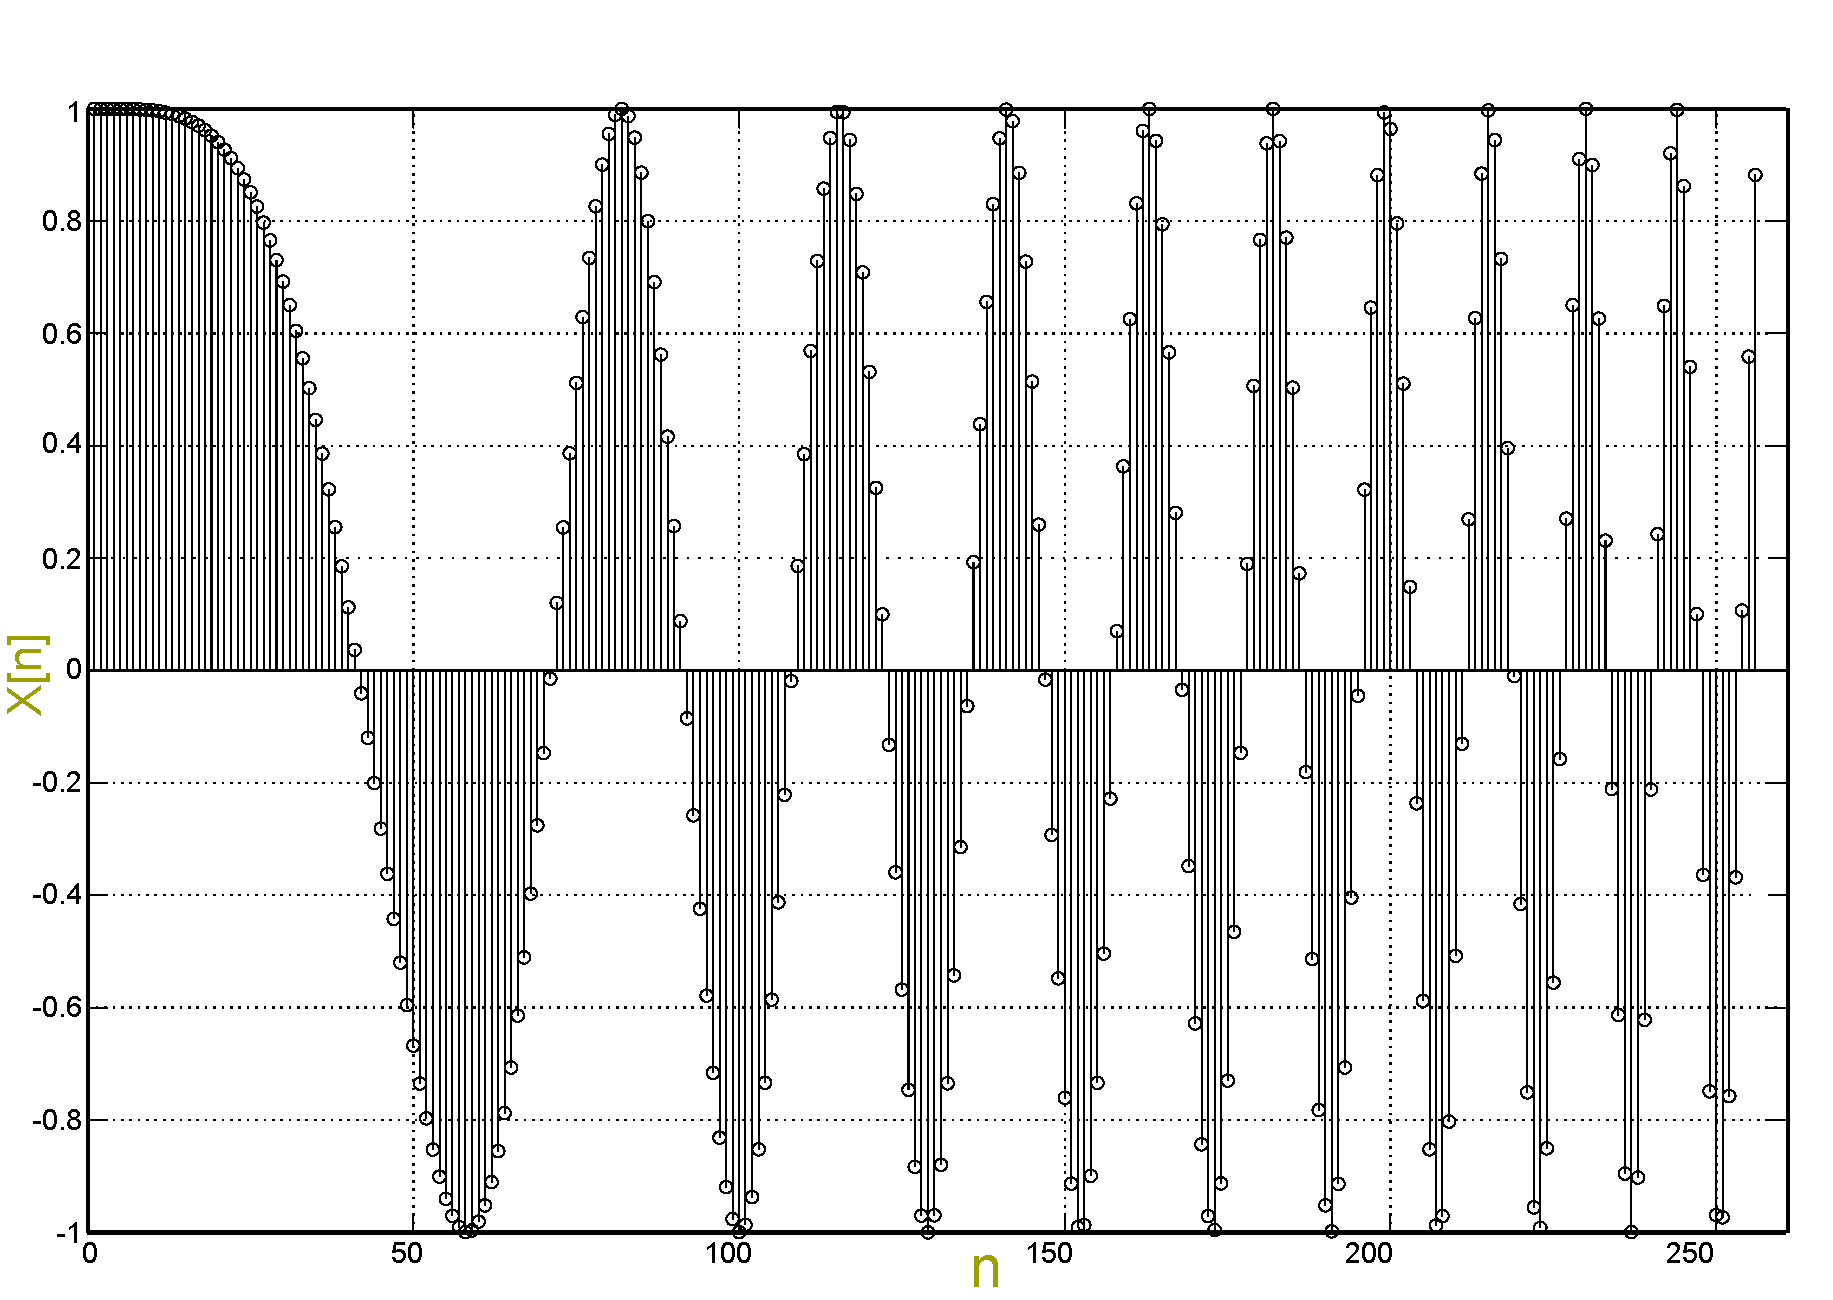
\includegraphics[width=0.8\linewidth]{Chirp_signal_stem.pdf} 
     \end{tabular}  
     \captionof{figure}{Chirp signál: Signál s lineárně rostoucím kmitočtem s maximální
              frekvencí 20 Hz vzorkovaný 254 Hz. Grafická reprezentace číslicových signálů bývá
              buď ve spojité formě (a) nebo v diskrétní formě (b) 
     \label{SAS:fig_chirp_sig}}
  \par}
  
  M-file:
  %---------------------------------------------------------------
  \lstinputlisting{../src/TKY/matlab/gen_chirp_signal.m}
  \begin{lstlisting}[caption=\texttt{gen\_chirp\_signal.m}. Generuje chirp signál]
  \end{lstlisting}
  %---------------------------------------------------------------
\end{example}
    %---------------------------------------------------------------

  \section{Základní operace s posloupnosti}
    V dalším textu budeme používat tři základní lineární operace \cite{Sovka} zobrazené na
    \ref{sas:fig_zakladni_operace}:
    \begin{itemize}
      \item \texttt{součin} signálu $x[n]$ a reálné konstanty $b$:      
            $$w[n]=bx[n], n = 0,1,2, \ldots$$ Tato operace je v praxi realizována násobičkou a je
            zdrojem numerických chyb, tedy kvantizačního šumu, který produkují číslicová zařízení.
      \item \texttt{součet} signálu $x[n]$ a signálu $y[n]$:           
            $$v[n]=x[n]+y[n], n = 0,1,2, \ldots$$ Tuto operaci provádí sčítačka. Při neošetření může
            tato operace generovat hrubé chyby.
      \item \texttt{zpoždění} signálu $x[n]$ o $k$ vzorkovacích kroků:  
            $$y[n]=x[n-k], n = 0,1,2, \ldots, n = 1,2, \ldots, M $$  Hodnoty $x[-k], k = 1, 2,
            \ldots, M$ se nazývají \emph{počáteční podmínky}. V digitálních implementací provádíme
            operaci zpoždění paměťového registru pro každou jednotku požadovaného zpoždění $z^{-1}$.
    \end{itemize}

    \begin{figure}[ht!]
      \centering
      \begin{tabular}{c}
        \hspace{0.1cm}
        \subfloat[ ]   {
          \begin{tikzpicture}[scale=1,>=latex']
  \coordinate (A) at (-1,-1.5) {};
  \coordinate (B) at (-1,-2.5) {};
  \coordinate (C) at (0,-2) {};    
  \coordinate (D) at ($ (A)!0.5!(B) $) {};
    \fill[fill=blue!20!white, draw=blue!50!black, very thick] (A) -- (B) -- (C) -- (A);
    \node[] at ($ (D)!0.4!(C) $) {\(b\)};
    \draw[->] (C) ++ (-2,0)  node[left] {\(x[n]\)} -- (D);
    \draw[->] (C) -+ (1,-2) node[right] {\(bx[n]\)}; 
\end{tikzpicture}}  \\
        \subfloat[ ]   {
          \begin{tikzpicture}[scale=1,>=latex']
  \coordinate (A) at (0,0) {};
  \coordinate (B) at (1,-1) {};   
  \coordinate (C) at ($ (A)!0.5!(B) $) {};   
  \coordinate (D) at (A |- C) {}; 
    \fill[fill=blue!20!white, draw=blue!50!black, very thick] (A) circle (0.5);
    \node[] at (A) {\(+\)};
    \draw[->] (-1.5,0) node[left] {\(x[n]\)} -- (-0.5,0);
    \draw[->] (0,1.5) node[above] {\(y[n]\)} -- (0,0.5);
    \draw[->] (0.5,0) --+ (1,0) node[right] {\(x[n]+y[n]\)}; 
\end{tikzpicture}
}  \\
        \subfloat[ ]   {
          \begin{tikzpicture}[scale=1,>=latex']
  \coordinate (A) at (0,0) {};
  \coordinate (B) at (1,-1) {};   
  \coordinate (C) at ($ (A)!0.5!(B) $) {};   
  \coordinate (D) at (A |- C) {}; 
    \fill[fill=blue!20!white, draw=blue!50!black, very thick] (A) rectangle (B);
    \node[] at (C) {\(z^{-k}\)};
    \draw[->] (D) + (-1,0) node[left] {\(x[n]\)} -- (D);
    \draw[->] (D) ++(1,0) --+ (1,0) node[right] {\(x[n-k]\)}; 
\end{tikzpicture}}    
      \end{tabular}
      \caption[Základní operace]{Symboly základních operací} 
      \label{sas:fig_zakladni_operace} 
    \end{figure}    

%---------------------------------------------------------------------------------------------------
\printbibliography[title={Seznam literatury}, heading=subbibliography]
\addcontentsline{toc}{section}{Seznam literatury}  
%======================= Kapitola: Popis spojitých a diskrétních systémů ===========================
  % !TeX spellcheck = cs_CZ
{\tikzset{external/prefix={tikz/TKY/}}
 \tikzset{external/figure name/.add={ch03_}{}}
%================== Kapitola: LTI systém ===========================================================
\chapter{LTI systém}
\minitoc
  \section{Vlastnosti a popis lineárních systému}
    \begin{wrapfigure}[8]{r}{5cm}
      \centering      
      \begin{tikzpicture}[scale=1,>=latex']
   \filldraw[fill=green!20!white, draw=green!50!black, very thick] (-1,1) rectangle (1,0);
   \coordinate (v1) at (-2,0.5);
   \coordinate (v2) at (-1,0.5);
   \coordinate (v3) at (1,0.5);
   \coordinate (v4) at (2,0.5);
   \draw[->] (v1) node[left] {\(x\)} -- (v2);
   \draw[->] (v3) --  (v4) node[right] {\(y\)} ; 
   \node[] at ($ (v2)!0.5!(v3) $) {\(S\)};
\end{tikzpicture}

      \caption[Symbol soustavy s jedním vstupem a jedním výstupem]{Symbol soustavy s jedním 
               vstupem a jedním výstupem}
      \label{sas:fig_soustava}   
    \end{wrapfigure}
    Na soustavu obvodů můžeme nahlížet jako na seskupení (množinu) navzájem souvisejících součástí, 
    ke kterému je určen vstupní signál $x$, zvaný buzení a výstupní signál $y$, označovaný jako 
    odezva. Z hlediska vlastností jde o systém představující "černou skříňku", jejíž vlastnosti 
    můžeme identifikovat analýzou vstupního a výstupního signálu \cite{Bicak}.
        
    \begin{itemize}
      \item Systémy se spojitým časem (na vstupu i výstupu pracují se spojitými signály) - relace  
            mezi vstupem a výstupem můžeme symbolicky zapsat:
            \begin{equation}\label{sas:eq_spojity_system}
              y(t)=\mathcal{S}\{x(t)\}
            \end{equation}
            kde $S$ je obecný popis systémové funkce, přiřazující vstupní veličině $x(t)$ odezvu 
            $y(t)$. Z rovnice je zřejmé, že u spojité (analogové) soustavy výstupní signál závisí 
            na všech hodnotách vstupního signálu, nikoli jen na některých jeho hodnotách v určitých 
            časových okamžicích.
      \item Systémy pracující s diskrétním časem lze obdobně symbolicky vyjádřit relací  
            vstup/výstup ve tvaru:
            \begin{equation}\label{sas:eq_dis_system}
              y[n]=\mathcal{S}\{x[n]\}
            \end{equation}
            kde $\mathcal{S}$ je tentokráte systémový operátor přiřazení posloupnosti 
            $x[n]\rightarrow y[n]$. U diskrétních systémů se zpracovávají posloupnosti hodnot 
            signálů, získaných vzorkováním spojitého signálu
    \end{itemize}
    
  \section{Linearita, časová invariance a kauzalita}
    \textbf{Linearita systémů} ve spojité diskrétní oblasti má velký význam, neboť dovoluje 
    využívat princip superpozice k zjednodušování úloh jejich analýzy  a syntézy.

    Předpokládejme, že na vstupu lineárního diskrétního systému jsou přivedeny dva signály $x_1[n]$ 
    a $x_2[n]$. Účinky obou vstupních signálů na výstupní signál lze zkoumat odděleně a podle 
    principu superpozice je na výstupu sečíst. Označme dílčí odezvy $y_1[n]=\mathcal{S}\{x_1[n]\}$ 
    a $y_2[n]=\mathcal{S}\{x_2 [n]\}$, potom je
    \begin{equation}\label{sas:eq_superpozice1}
      y[n]= y_1[n]+y_2[n]=S\{x_1[n]+x_2[n]\}
    \end{equation}
    Analogický vztah platí i pro lineární spojitý systém, tedy
    \begin{equation}\label{sas:eq_superpozice2}
      y(t)= y_1(t)+ y_2(t)=S\{x_1(t)+x_2(t)\}
    \end{equation}
    Jedná-li se o \emph{systém časově invariantní}, jsou události v čase závislé pouze na časovém
    intervalu (rozdílu časových událostí), nikoliv na každém časovém okamžiku sa\-mos\-tat\-ně. 
    Systém je časově invariantní, jestliže časový posun ve vstupní signálu vede ke stejnému posunu 
    výstupního signálu. Odezva diskrétního systému na posunutý vstupní signál $x[n-m]$ je pak určen 
    vztahem
    \begin{equation}\label{sas:eq_odezva1}
      y[n-m]= \mathcal{S}\{x[n-m]\}
    \end{equation}
    a obdobně pro odezvu spojité soustavy na posunutý (zpožděný) vstupní signál $x(t-\tau)$ platí
    analogicky rovnice
    \begin{equation}\label{sas:eq_odezva2}
      y(t-\tau)= \mathcal{S}\{x(t-\tau)\}.
    \end{equation}
    \textbf{Kauzální, příčinný systém} je systém, u kterého výstupní signál závisí pouze na 
    současných a minulých hodnotách vstupního signálu.

    \subsection{Konvoluce v diskrétních a spojitých systémech}
      \cite{Bicak} Významnou charakteristikou lineárních časově invariantních systémů \emph{LTI} je
      \textbf{impulzní odezva}. Její znalost umožňuje stanovit odezvu systému na obecný signál, lze 
      ji využít i při syntéze systému.
      \begin{equation}\label{sas:eq_odezva3}
        h[n]= \mathcal{S}\{\delta[n]\}.
      \end{equation}
      Mějme diskrétní LTI systém, na jehož vstup je přiveden \emph{jednotkový diskrétní      
      impulz}\footnote{Nesmíme zaměňovat s Diracovým (také jednotkovým) impulzem.}. Jednotkový 
      impulz je posloupnost $\delta[n]=0$ pro všechna $n$ s výjimkou $\delta[0]=1$. Odezva systému 
      na jednotkový impulz $\delta[n]$ se nazývá impulzní odezva a platí
      \begin{equation}\label{sas:eq_odezva_posun}
        h[n-m]= \mathcal{S}\{\delta[n-m]\}.
      \end{equation}
      Vzhledem časové invariantnosti, posunutému jednotkovému impulzu odpovídá posunutá impulzní
      odezva, tedy
      \begin{equation}\label{sas:eq_jednotkovy_skok}
        1[n]= \sum_{m=0}^n[n-m] =\delta[n]+\delta[n-1]+\delta[n-2]+\cdots.
      \end{equation}
      \emph{Jednotkový skok} $\mathrm{1}[n]$ je posloupnost jedniček od počátku časové osy $n=0$,
      kterou můžeme zapsat součtem
      \begin{equation}\label{sas:eq_odezva_skok}
        s[n]= \mathcal{S}\{\mathrm{1}[n]\}=S\{\sum_{m=0}^n[n-m]\}=\sum_{m=0}^nS\{\delta[n-m]\}.
      \end{equation}
      \emph{Odezva systému na jednotkový skok} $\mathrm{1}[n]$ se nazývá \textbf{přechodová odezva}
      $s[n]$ a platí
      \begin{equation}\label{SAS:eq_odezva_skok2}
        s[n]=\mathcal{S}\{\sum_{m=0}^n\delta[n-m]\}=\sum_{m=0}^n\mathcal{S}\{\delta[n-m]\}.
      \end{equation}
      Odezva kauzálního diskrétního systému na jednotkový impulz $\delta[n]$, resp. na posunutý
      impulz $\delta[n-m]$, bude  $h[n]$  resp.  $h[n-m]$ - viz obr. \ref{SAS:fig_odezva3}.
      \begin{figure*}[ht!]
        \centering
        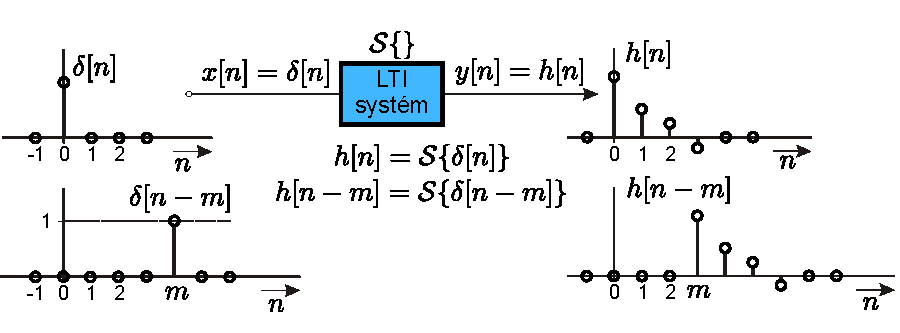
\includegraphics[scale=0.8]{impulzni_odezva.pdf}
         \caption[Impulzní odezva]{Odezva kauzálního diskrétního systému na jednotkový impulz
                  $\delta[n]$ a posunutý impulz $\delta[n-m]$}
        \label{SAS:fig_odezva3}
      \end{figure*}
  
      Postupná úprava rovnice (\ref{SAS:eq_odezva_skok2}) je umožněna díky linearitě systému,
      kterou budeme studovat pro obecný vstupní signál
      \begin{equation}\label{SAS:eq_odezva_na_diskretni_signal}
        x[n]=\sum_{m=-\infty}^\infty x[m]\delta[n-m].
      \end{equation}
      Poznamenejme, že formou (\ref{SAS:eq_odezva_na_diskretni_signal}) lze zapsat každý diskrétní
      signál.
     
      %---------------------------------------------
      \pgfplotsset{
    standard/.style={%Axis format configuration
        axis x line=middle,
        axis y line=middle,
        enlarge x limits=0.15,
        enlarge y limits=0.15,
        every axis x label/.style={at={(current axis.right of origin)},anchor=north west},
        every axis y label/.style={at={(current axis.above origin)},anchor=north east},
        every axis plot post/.style={mark options={fill=white}}
        }
  }
  \begin{figure}[hb!]
    \centering
    \subfloat[ ]   { %Unit step squence
      \begin{tikzpicture}
        \begin{axis}[%
          scale=0.45,
          standard,
          domain = 0:15,
          samples = 16,
          xlabel={\(n\)},
          ylabel={\(1[n]\)},
          ymin=0,
          ymax=1.1]
          \addplot+[ycomb,blue,thick] {1};
        \end{axis}
      \end{tikzpicture}
    }
    \subfloat[ ]   { %Sampled sine squence
      \begin{tikzpicture}
         \begin{axis}[%
            scale=0.45,
            standard,
            domain = 0:15,
            samples = 16,
            xlabel={$n$},
            ylabel={$x[n]$},
            ymax=1.1]
            \addplot+[ycomb,blue,thick] {sin(5*180*x/25)};
         \end{axis}
      \end{tikzpicture}
    }
    \caption[Posloupnost jednotkového a obecného signálu]{Posloupnost jednotkového skoku $1[n]$
             a signálu $x[n]$}
    \label{SAS:fig_odezva4}    
  \end{figure}

      % \label{SAS:fig_odezva4}
      %---------------------------------------------
      
      Na obr. \ref{SAS:fig_odezva4} znázorněna souvislost mezi posloupností jedniček a diskrétním
      sig\-ná\-lem. \emph{Posloupnost jedniček tvoří bázi pro diskrétní signály}. Každá komponenta
      diskrétního signálu je vyjádřena součinem $x[m]\delta[n-m]$. V uvedeném příkladě jde o
      posloupnost příslušnou jednotkovému skoku
      \begin{equation}\label{SAS:eq_odezva5}
        1[n]=\sum_{m=0}^{15}\delta[n-m]
      \end{equation}
      a odpovídající posloupnost konečného signálu
      \begin{equation}\label{SAS:eq_odezva6}
        x[n]=\sum_{m=0}^{15}x[m]\delta[n-m].
      \end{equation}
  
      Princip superpozice dovoluje získat odezvu systému jako sumu odezev na jednotlivé dílčí
      součásti vstupního signálu, které v rovnici (\ref{SAS:eq_odezva_na_diskretni_signal}) tvoří
      vážené jednotlivé impulzy, ze kterých je signál složen
      \begin{align}
        y[n]=\mathcal{S}\{x[n]\}
          &=\mathcal{S}\{\sum_{m=-\infty}^{\infty}x[m]\delta[n-m]\}  \nonumber \\
          &=\sum_{m=-\infty}^{\infty}x[m]\mathcal{S}\{\delta[n-m]\}. \label{SAS:eq_odezva7}
      \end{align}
      Protože platí (\ref{sas:eq_odezva3}) a v důsledku časové invariance vyplývá z rovnice
      \ref{SAS:eq_odezva7} \textbf{konvoluční suma} 
      \begin{equation}\label{SAS:eq_konvolucni_suma}
        y[n]=\sum_{m=-\infty}^{\infty}h[n-m]x[m]=\sum_{k=-\infty}^{\infty}h[k]x[n-k].
      \end{equation}
      Uvedli jsme, že u kauzálního systému závisí výstupní signál $y[n]$ pouze na současných a
      minulých hodnotách vstupního signálu $x[n], x[n-1], x[n-2], \cdots ,$ takže v konvoluční sumě
      \ref{SAS:eq_konvolucni_suma}
      \begin{align}
        y[n]&=\sum_{k=-\infty}^{\infty}h[k]x[n-k]                              \nonumber \\
            &=\sum_{k=-\infty}^{-1}h[k]x[n-k] + \sum_{k=0}^{\infty}h[k]x[n-k]  \label{tky:eq001}
      \end{align}
      musíme položit všechny členy impulzní odezvy $h[k]=0$ pro $k<0$. Konvoluční suma pro
      lineární, časově invariantní a kauzální systém má pak tvar
      \begin{equation}\label{SAS:eq_konvolucni_suma3}
        y[n]=\sum_{k=0}^{\infty}h[k]x[n-k].
      \end{equation}
      Jestliže navíc budeme uvažovat vstupní a výstupní signály, které jsou nulové pro $n<0$ a
      $x[n]\neq0, y[n]\neq0$ pouze pro $n\geq0$, potom platí
      \begin{equation}\label{SAS:eq_konvolucni_suma4}
        y[n]=\sum_{k=0}^{n}h[k]x[n-k]=\sum_{k=0}^{n}x[k]h[n-k].
      \end{equation}
  
      \begin{figure}[ht!]
        \centering
        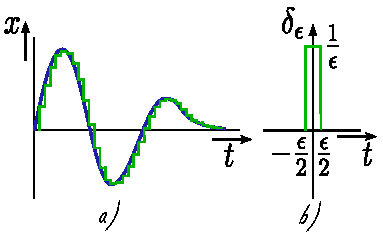
\includegraphics[width=0.7\linewidth]{bicak_aprox_spoj_sig_dirac.pdf}
        \caption[Aproximace spojitého průběhu signálu]{a) Aproximace spojitého průběhu signálu, b)
                 K odvození jednotkové impulsní funkce}
        \label{SAS:fig_Bicak_aprox_spoj_fce}
      \end{figure}
  
      Podobně můžeme postupovat i v analogovém případě a odvodit pro lineární časově invariantní 
      systém \emph{konvoluční integrál}. Vraťme se k výrazu \ref{SAS:eq_odezva_na_diskretni_signal} 
      kterým jsme vyjádřili libovolný diskrétní signál. Pro případ spojitého signálu vytvořme 
      analogickou formu zápisu využívající jednotkový impuls. Průběh obecného spojitého lze podle 
      obr. \ref{SAS:fig_Bicak_aprox_spoj_fce} aproximovat stupňovitým průběhem, který můžeme 
      vyjádřit jako sumu posunutých (zpožděných) impulsů. Výchozí aproximující impuls lze vyjádřit 
      vztahem
      \begin{equation}\label{SAS:eq_dirac}
          \delta_\epsilon(t)  =
            \begin{cases}
               \frac{1}{\epsilon} & \text{pro } |t| < \frac{\epsilon}{2},      \\
               0                  & \text{pro } |t| < \frac{\epsilon}{2} > 0
            \end{cases}
      \end{equation}
      a je znázorněn na obr. \ref{SAS:fig_Bicak_aprox_spoj_fce}. \emph{Jednotkový (Diracův) impuls} 
      má jednotkovou plochu. vat výrazem
      \begin{equation}\label{SAS:eq_dirac2}
        \delta_\epsilon(t) = \lim_{\epsilon\rightarrow0} \delta_\epsilon(t).
      \end{equation}
      Aproximaci spojitého průběhu $x(t)$ impulsy \ref{SAS:eq_dirac} lze vyjádřit rovnicí
      \begin{equation}\label{SAS:eq_spojit_aprox}
        x(t) = \sum_{m = -\infty}^\infty x(m\epsilon)\delta_\epsilon(t - m\epsilon)\epsilon .
      \end{equation}
      Zmenšování šířky impulsů $\epsilon \rightarrow 0$ se chyba aproximace zmenšuje a výraz přejde v limitu
      \begin{equation}\label{SAS:eq_spojit_aprox2}
        x(t) = \lim_{\epsilon\rightarrow0}
               \sum_{m = -\infty}^\infty x(m\epsilon)\delta_\epsilon(t - m\epsilon)\epsilon .        
      \end{equation}
      V limitě kdy $\epsilon\rightarrow0$, můžeme sumu nahradit integrálem, dále součin $m\epsilon$ 
      integrační proměnnou $\tau$ a $\epsilon$ jejím diferenciálem. Obdržíme
      \begin{equation}\label{SAS:eq_integral_aprox3}
        x(t) = \int_{-\infty}^{\infty}x(\tau)\delta(t-\tau)d\tau .
      \end{equation}
      Vztahem \ref{SAS:eq_integral_aprox3} jsme spojitý průběh signálu vyjádřili jako sumu 
      nekonečného počtu posunutých jednotkových impulsů váženou jeho okamžitými hodnotami. 
      Předpokládejme dále, že na vstup lineárního časově invariantního spojitého systému je 
      převeden jednotkový (Diracův) impuls a systém vytvoří odezvu $h(t)$. V případě obecného 
      vstupního spojitého signálu $x(t)$ aproximovaného vztahem \ref{SAS:eq_integral_aprox3}, bude 
      odezva analogového systému
      \begin{equation}\label{SAS:eq_integral_aprox4}
        y(t) = \int_{-\infty}^{\infty}x(\tau)h(t-\tau)d\tau 
             = \int_{-\infty}^{\infty}h(\tau)x(t-\tau)d\tau
      \end{equation}
      Uvedený integrál nazýváme \textbf{konvolucí} a velmi často ho označujeme jako 
      \begin{equation}\label{SAS:eq_konvoluce}
        y(t) = h(t)*x(t) .
      \end{equation}
      Funkce $h(t)$ představuje \emph{impulsní odezvu}. Jedná se o výstupní signál systému, na 
      jehož vstupu se uplatní Diracův impuls $x(t)=\delta(t)$. Platí totiž
      \begin{equation}\label{SAS:eq_h_plati}
        y(t) = \int_{-\infty}^{\infty}h(\tau)\delta(t-\tau)d\tau = h(t) . 
      \end{equation}     
      Z důvodů \emph{kauzality}, která vyjadřuje zachování příčinné posloupnosti událostí při 
      transformaci signálu ze vstupu na výstup, požadujeme
      \begin{align}\label{SAS:eq_kauzalita_pozadavky}
        h(t) &\neq  0 \text{   pro } |t| \geq0, \\
        h(t) &  =   0 \text{   pro } |t| < 0. 
      \end{align}    
      Potom můžeme konvoluční integrál \ref{SAS:eq_integral_aprox4} zapsat ve tvarem
      \begin{equation}\label{SAS:eq_konvolucni_integral}
         y(t) = \int_0^{\infty}h(\tau)x(t-\tau)d\tau .
      \end{equation} 
  
  \section{Popis spojitých a diskrétních systémů, pře\-no\-so\-vá funkce}
    \subsection{Spojité systémy}
      Lineární časově invariantní (LTI) spojitý systém je obecně popsán soustavou
      integrodiferenciálních rovnic s konstantními koeficienty, kterou lze postupným derivováním
      změnit na soustavu diferenciálních rovnic. Předpokládej\-me budící (ne\-zá\-vis\-lou) veličinu
      $x(t)$ a odezvou (závislou) výstupní veličinu $y(t)$, pak eliminací ostatních proměnných bude 
      soustava popsána jedinou diferenciální rovnicí s konstantními koeficienty tvaru
      \begin{equation}\label{SAS:eq_lin_dif_rov}
          \sum_{i=0}^na_i\frac{d^iy(t)}{dt^i}=\sum_{j=0}^mb_j\frac{d^jx(t)}{dt^j},
      \end{equation}
      kde $a_0, a_1, \cdots ,a_n$ a $b_0, b_1, \cdots ,b_m$ jsou konstanty charakterizující lineární
      systém. Obecné řešení $y(t)$ rovnice \ref{SAS:eq_lin_dif_rov} se sestává ze dvou částí, z 
      řešení \emph{homogenní rovnice} a \emph{partikulárního řešení}. K řešení je třeba znát 
      počáteční podmínky pro $y(t)$ a jeho derivace ve výchozím okamžiku.
  
      S použitím \emph{Laplaceovy transformace při nulových počátečních podmínkách} má rovnice
      (\ref{SAS:eq_lin_dif_rov}) tvar
      \begin{equation}\label{SAS:eq_L_tran_dif_rce}
        \sum_{i=0}^na_ip^iY(p)=\sum_{j=0}^mb_jp^jX(p),
      \end{equation}
      kde $X(p)=\mathcal{L}\{x(t)\}$ a $Y(p)=\mathcal{L}\{y(t)\}$ jsou Laplaceovy obrazy vstupní a
      výstupní veličiny, $p$ je Laplaceův operátor derivace a také komplexní kmitočet 
      $p=\sigma+j\omega$. Přenosová funkce $H(p)$ je definována jako podíl Laplaceova obrazu 
      výstupní veličiny $Y(p)$ ku obrazu vstupní veličiny $x(p)$, při nulových počátečních 
      podmínkách
      \begin{equation}\label{SAS:eq_Hp_popis}
          H(p)=\frac{Y(p)}{X(p)}.
      \end{equation}
      Vzhledem k rovnici (\ref{SAS:eq_L_tran_dif_rce}) je $H(p)$ racionálně lomenou funkcí tvaru
      \begin{align}
        H(p)&=\frac{b_mp^m+b_{m-1}p^{m-1}+\cdots+b_0}{a_np^n+b_{n-1}p^{n-1}+\cdots+a_0}  \nonumber\\
            &=\frac{\Pi_{j=1}^m(p-p_{0j})}{\Pi_{i=1}^n(p-p_{\infty i})}            \label{tky:eq002}
      \end{align}
      kde $p_{0j}$ jsou kořeny polynomu čitatele a představují \textbf{nulové body} a kořeny
      jmenovatele $p_{\infty i}$ jsou \textbf{póly} přenosové funkce, $H_0=\frac{b_m}{a_n}$ je
      násobná konstanta.
  
      Kmitočtové charakteristiky získáme z přenosové funkce substitucí
      \begin{equation}\label{SAS:eq_p_jomega}
          p = j\omega,
      \end{equation}
      ve které $\omega$ je úhlový kmitočet. Platí tedy
      \begin{align}
          H(p)\mid_{p = j\omega} 
            &=\frac{b_m(j\omega)^m+b_{m-1}(j\omega)^{m-1}                     
             +\cdots+b_0}{a_n(j\omega)^n+b_{n-1}(j\omega)^{n-1}+\cdots+a_0}      \nonumber \\
            &=M(\omega)e^{j\Phi(\omega)},                                        \label{tky:eq003}
      \end{align}
      kde $M(\omega)$ je \textbf{modulová charakteristika} a $\Phi(\omega)=\texttt{arg}H(j\omega)$ 
      se nazývá \textbf{fázová charakteristika}. Skupinové zpoždění je definováno jako záporně vzatá
      derivace fázové charakteristiky podle kmitočtu
      \begin{equation}\label{SAS:eq_skupinove_zpozdeni}
          \tau(\omega)=-\frac{d\Phi(\omega)}{d\omega}= - \frac{d \texttt{arg} H(j\omega)}{d\omega}.
      \end{equation}
      V předchozí kapitole jsme ukázali, že \emph{relace vstup/výstup LTI systému} souvisí
      pro\-střed\-nic\-tvím \emph{konvoluce}
      \begin{equation}\label{SAS:eq_popis_konvoluce}
          y(t)=\int_0^\infty h(\tau)x(t-\tau)d\tau = h(t)*x(t).
      \end{equation}
      Přenosová funkce je Laplaceova transformace impulzní odezvy $h(t)$
      \begin{equation}\label{SAS:eq_ht_Lap_trans_imp}
          H(p)=\mathcal{L}[h(t)]=\int_0^\infty h(t)e^{-pt}dt,
      \end{equation}
      pro kterou je splněn vztah
      \begin{equation}\label{SAS:eq_Yp}
          Y(p)=H(p)X(p).
      \end{equation}
      Přechodová odezva $s(t)$ je definována jako integrál impulzní odezvy
      \begin{equation}\label{SAS:eq_Prechod_odezva}
          s(t)=\int_0^th(\tau)d\tau,
      \end{equation}
      takže platí
      \begin{equation}\label{SAS:eq_st}
          s(t)=\mathcal{L}^{-1}\{\frac{H(p)}{p}\}.
      \end{equation}
      Algoritmus výpočtu impulzní odezvy z přenosové funkce je založen na výpočtu  reziduí a 
      rozkladu racionálně lomené funkce $H(p)=\frac{Q(p)}{N(p)}$ na částečné zlomky. Pokud má tato 
      funkce jednoduché póly, rozklad má tvar\footnote{Násobnost kořenů $N(p)$ neuvažujeme, protože 
      se v LTI obvodech neuplatňuje}.
      \begin{align}   %\label{tky:eq004}
         H(p)&=\frac{Q(p)}{N(p)} 
              =\sum_{\mu=1}^{n}\frac{k_\mu}{p-p_{\infty_\mu}}                  \nonumber \\
             &=\frac{k_1}{p-p_{\infty_1}}+\frac{k_2}{p-p_{\infty_2}}
               +\cdots+\frac{k_n}{p-p_{\infty_n}}                              \label{tky:eq004}
      \end{align}
      kde $k_\mu$ se nazývají rezidua v pólech $p_{\infty_\mu})$ a platí
      \begin{align}
        k_\mu &= \lim_{p\to p_{\infty_\mu}}(p-p_{\infty_\mu})\frac{Q(p)}{N(p)}  \nonumber \\
        \,    &= Q(p_{\infty_\mu})\lim_{p\to
                 p_{\infty_\mu}}\frac{1}{\frac{N(p)}{p-p_{\infty_\mu}}}=
                 Q(p_{\infty_\mu})\frac{1}{N'(p_{\infty_\mu})}                  \label{tky:eq006}
      \end{align}
      Impulzní odezva je pak dána vztahem
      \begin{equation}\label{sas:eq_impulzni_odezva}
        h(t)=\mathcal{L}^{-1}[H(p)]=\sum_{\mu=1}^nk_\mu e^{p_{\infty_\mu}t}
      \end{equation}
      Póly jsou obecně komplexní $p_{\infty_{\mu}}=\alpha_\mu+j\beta_\mu$, nebo reálné
      $p_{\infty_{\mu}}=\alpha_\mu$. Jsou to kořeny rovnice $N(p)=0$. Rovnice
      \ref{sas:eq_impulzni_odezva} je důležitá i proto, že z ní poznáme, zda analogová soustava je
      stabilní. Je patrné, že soustava bude stabilní, jestliže bude
      $\mathcal{R}\{p_{\infty_{\mu}}\}=\alpha_\mu<0$, tj. leží-li kořeny $p_{\infty_{\mu}}$ v
      otevřené levé polorovině komplexní roviny $p_{\infty_{\mu}}=\sigma+j\omega$. Imaginární osa
      $j\omega$ je mezí stability, pravá polorovina je oblastí nestability. Polynom, který má kořeny
      v levé otevřené polorovině se označuje \textbf{Hurwitzův polynom}.
      %---------------------------------------------------------------
      % !TeX spellcheck = cs_CZ
% Lineární obvody a systémy - Jan Bičák  - strana 10
% Popis spojitých systémů
%===================================================================================================
\begin{example}Lineární spojitý systém je dán zapojením dle obrázku. Určete:
  \begin{enumerate}
    \item diferenciální rovnici pro odezvu $u_2(t)$, je-li na vstupu buzen napětím $u_1(t)$,
    \item přenos napětí $H(p)=\dfrac{U_2(p)}{U_1(p)}$,
    \item impulsní odezvu $h(t)$.
  \end{enumerate}

   {\centering
    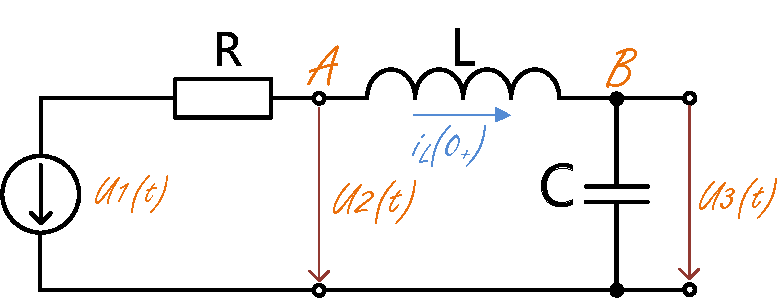
\includegraphics[scale=0.5]{cir_RLC.pdf}
    \captionof{figure}{Zapojení obvodu RLC.}
    \label{SAS:fig_RLC}
    \par}
  \textbf{Řešení:}\newline
  Pro zapojení dle obrázku získáme metodou uzlových napětí integrodiferenciální rov\-ni\-ce pro
  uzly \texttt{A} a \texttt{B}:
  \begin{align}\label{SAS:eq_RLC_basic_rces}
    A &:  \frac{u_3(t)-u_1(t)}{R}+\frac{1}{L}
    \int_0^t{(u_3(t)-u_2(t))}d\tau+i_L(0_+) = 0\,               \\ \nonumber
    B &:  \frac{1}{L}\int_0^t{(u_2(t)-u_3(t))}d\tau+C\frac{du_c}{dt}-i_L(0_+)        = 0
  \end{align}
  Derivováním a eliminací $u_3(t)$ z původních rovnic dostaneme pro odezvu $u_2(t)$ diferenciální
  rovnici II. řádu
  \begin{itemize}
    \item \(\frac{d}{dt}(B)\):
          \begin{equation*}
            u_2(t)-u_3(t)+LC\frac{d^2u_2(t)}{dt^2}
            =0\Rightarrow u_3(t)=u_2 (t)+LC\frac{d^2u_2(t)}{dt^2}
          \end{equation*}
    \item \(\frac{d}{dt}(B)\rightarrow(A)\):
  \end{itemize}
  \begin{align*}
    \frac{u_2(t)+LC\frac{d^2u_2(t)}{dt^2}-u_1(t)}{R}+
    \frac{1}{L}\int_0^t{(LC\frac{d^2u_2(t)}{dt^2})}d\tau+i_L(0_+) &=  0 \\
    u_2(t)+LC\frac{d^2u_2(t)}{dt^2}-u_1(t)+
    RC\left[\frac{du_2(t)}{dt}\right]_0^t+Ri_L(0_+)               &=  0
  \end{align*}
  Při nulových počátečních podmínkách: $\frac{du_2(t)}{dt}|_{t=0}=0$, $i_L(0_+)=0$ dostaneme:
  \begin{equation}\label{sas:eq_dif_RLC_II_r}
    LC\frac{d^2u_2(t)}{dt^2}+RC\frac{du_2(t)}{dt}+u_2(t)=u_1(t)
  \end{equation}
  V Laplaceově transformaci platí:
  \begin{align*}
    \mathcal{L}\left[\frac{du_2(t)}{dt}\right]     &= pU_2(p)-u_2(0) \\
    \mathcal{L}\left[\frac{d^2u_2(t)}{dt^2}\right] &= p^2U_2(p)-pu_2(0)-u_2(0),\,kde\,u_2(0)=
    \frac{du_2(t)}{dt}|_{t=0}
  \end{align*}
  při nulových počátečních podmínkách
  \begin{equation}\label{sas:eq_L_RLC_rce}
    p^2LCU_2(p)+pRCU_2(p)+U_2(p)=U_1(p)
  \end{equation}
  Odtud vyplývá \textbf{přenosová funkce} $H(p)=\frac{U_2(p)}{U_1(p)}$
  \begin{equation}\label{sas:eq_Hp_RLC}
    H(p)=\frac{1}{p^2LC+pRC+1}
        =\frac{1}{LC}\frac{1}{p^2+p\frac{R}{L}+\frac{1}{LC}}=\frac{Q(p)}{N(p)}
  \end{equation}
  K nalezení \textbf{impulsní odezvy} nejprve určíme póly přenosové funkce řešením rovnice
  $N(p)=0$
  \begin{equation}\label{sas:eq_koreny_L_rce}
    p_{\infty_{12}}=\frac{\frac{R}{L}\pm\sqrt{\left(\frac{R}{L}\right)^2-\frac{4}{LC}}}{2}
    =\frac{R}{2L}\pm\sqrt{\left(\frac{R}{2L}\right)^2-\frac{1}{LC}}
  \end{equation}
  přenosovou funkci pak upravíme do tvaru
  \begin{equation}\label{sas:eq_Hp_forma}
    H(p)=\frac{K}{(p-p_{\infty_1})\cdot(p-p_{\infty_2})}, \qquad K=\frac{1}{LC}
  \end{equation}
  \begin{itemize}
    \item Uvažujeme-li jednoduché póly a bude-li $R>2\sqrt{\frac{L}{C}}$ , potom z  rov.
          \ref{sas:eq_koreny_L_rce} vyplývají dva reálné různé póly. Přenosovou funkci tedy můžeme
          zapsat obecným tvarem:
          \begin{equation}\label{sas:eq_Hp_forma_2}
            H(p)=\frac{K}{(p+a_1)\cdot(p+a_2)}=\frac{k_1}{p+a_1}+\frac{k_2}{p+a_2}
          \end{equation}
          kde $p_{\infty_1}=-a_1,\, p_{\infty_2}=-a_2$, Rezidua  $k_1=\frac{K}{a_2-a_1}$,
          $k_2=\frac{K}{a_1-a_2}$ určíme z rov. \ref{sas:eq_HP_rezidua}. Impulsní odezvu pak
          vypočteme užitím rov. \ref{sas:eq_impulzni_odezva}.
          \begin{equation}\label{sas:eq_ht1}
            h(t)=\mathcal{L}^{-1}[H(p)]=\frac{K}{a_2-a_1}e^{-a_1t}+\frac{K}{a_1-a_2}e^{-a_2t}
          \end{equation}
    \item Když bude $R<2\sqrt{\frac{L}{C}}$, obdržíme dvojici komplexně sdružených pólů a
          pře\-no\-so\-vou funkci může obecně zapsat takto:
          \begin{equation}\label{sas:eq_ht2}
            H(p)=\frac{K}{(p+a_1)\cdot(p+a_2)}=\frac{k_1}{p+a-jb}+\frac{k_2}{p+a+jb}
          \end{equation}
          kde $p_{\infty_1}=-a+jb$, $p_{\infty_2}=-a-jb$. Rezidua v pólech jsou dány výrazy
          $k_1=-\frac{jK}{2b}$, $k_2=\frac{jK}{2b}$. Impulzní odezvu opět určíme užitím rov.
          \ref{sas:eq_impulzni_odezva}.
          \begin{equation*}
            h(t) = \frac{Ke^{-at}}{2b}\left[j\cdot\left(-e^{jbt}+e^{-jbt}\right)\right]
          \end{equation*}
          \begin{align}
            \,  &= \frac{Ke^{-at}}{2b}\left[j\cdot
            \left(\underline{-\cos(bt)}-j\sin(bt)+
            \underline{\cos(bt)}-j\sin(bt)\right)\right]                        \nonumber\\
            \,  &= \frac{K}{b}e^{-at}\sin(bt)                                   \label{tky:eq005}
          \end{align}
  \end{itemize}
  
  Pro stavební prvky: $R=1k\Omega, L=11.5mH, C=22.5nF$ ukazuje výpis m-file  
  \texttt{SAS\_exam\_02\_symb\_Hp\_solve.m} symbolický způsob řešení operátorových
  ob\-vo\-do\-vých rovnic pomocí \texttt{MATLABu}. Jde o typ \textbf{dolní propust}, jehož
  přenosová funkce má tvar: $$H(p)= \frac{3.9506\cdot10^9}{p^2+8.8889\cdot10^4p+3.9506\cdot10^9}.$$
  %---------------------------------------------------------------
  \lstinputlisting{../src/TKY/matlab/SAS_exam_02_symb_Hp_solve.m}
  \begin{lstlisting}[caption=TKY\_exam\_02\_symb\_Hp\_solve.m]
  \end{lstlisting}
  %--------------------------------------------------------------
  Impulzní charakteristiku obdržíme dosazením do vztahu \ref{tky:eq005}
  $$h(t)=\frac{K}{b}e^{-at}\sin(bt) 
  =8.8890\cdot10^4e^{-4.4444\cdot10^4t}\sin(4.4444\cdot10^4t).$$
  
    {\centering
    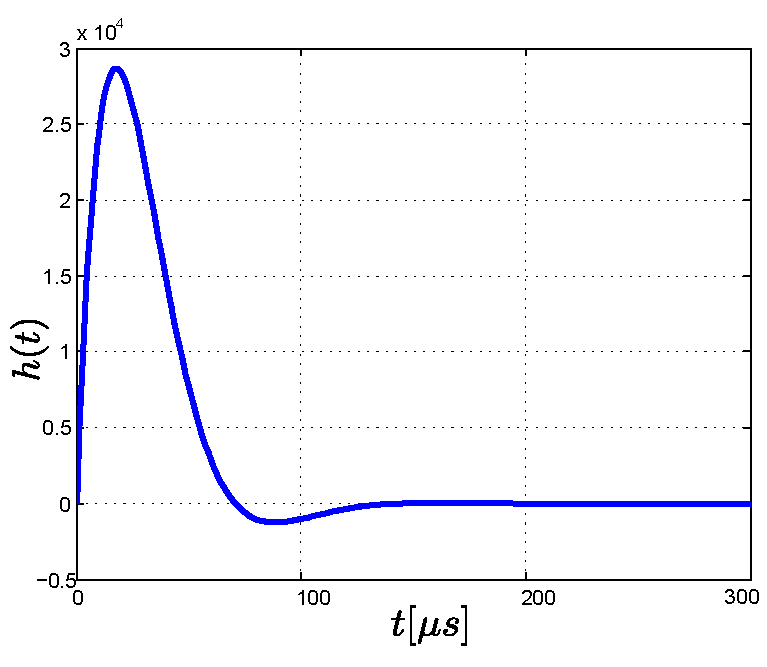
\includegraphics[scale=0.7]{ht.pdf}
    \captionof{figure}{Impulzní charakteristika}
    \label{SAS:fig_ImpChar}
    \par}
  
  Z hlediska analýzy obvodů v kmitočtové oblasti je výhodné sestavovat obvodové rovnice (metodami
  uzlových napětí a smyčkových proudů) přímo v operátorovém tvaru. Kirchhoffovy zákony pro
  uzavřenou smyčku a proudu do uzlu pak mají tvar $$\sum_{k=1}^{n}U_k(p) = 0, \qquad
  \sum_{k=1}^{n}I_k(p) = 0.$$ Metodou uzlových napětí pro zapojení na obr. \ref{SAS:fig_RLC}
  obdržíme rovnice
  \begin{align}
    \frac{U_3(p)-U_1(p)}{R}+\frac{U_3(p)-U_2(p)}{pL} &=  0 \\
    pCU_2(p) + \frac{U_2(p)-U_3(p)}{pL}              &=  0 
  \end{align}
  Na rozdíl od \ref{SAS:eq_RLC_basic_rces} jde o algebraické rovnice, ze kterých eliminací
  uzlového napětí $U_3(p)$ vyplývá přenosová funkce \ref{sas:eq_Hp_RLC} $$H(p) =
  \frac{U_2(p)}{U_1(p)}=\frac{1}{LC}\frac{1}{p^2+p\frac{R}{L}+\frac{1}{LC}}$$
  
   {\centering
    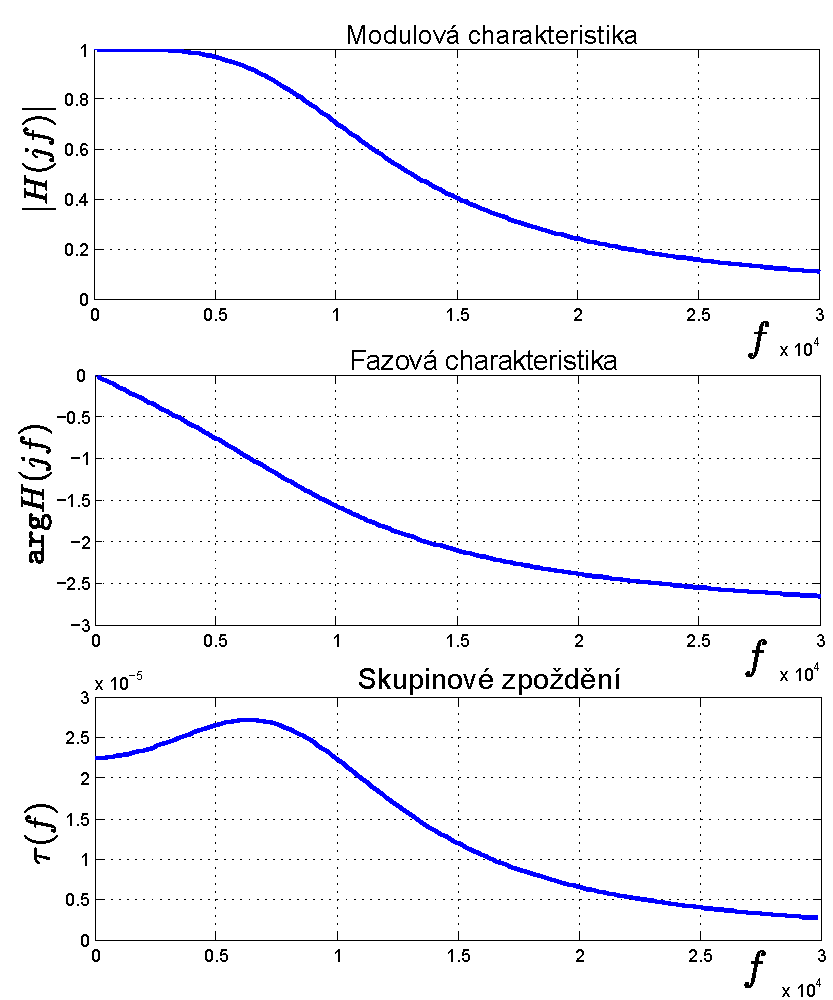
\includegraphics[width=0.7\linewidth]{cir_RLC_response_H_PHA_GD.pdf}
    \captionof{figure}{Modulová, fázová charakteristika a skupinové zpoždění filtru}
    \label{SAS:fig_ex01_RLC}
    \par}    
  
  Dosazením za $p=j\omega$ lze z přenosové funkce vyjádřit modulovou charakteristiku $H(j\omega)$
  a fázovou charakteristiku $\Phi(\omega)= \texttt{arg} H(j\omega)$. Skupinové zpoždění vyplývá
  ze vztahu \ref{SAS:eq_skupinove_zpozdeni}. Modulová, fázová charakteristika a skupinové
  zpoždění jsou na obr. \ref{SAS:fig_ex01_RLC}.
  
  Filtr má maximálně plochou modulovou charakteristiku přenosu. Mezní kmitočet propustného pásma
  je $f_p = 10 kHz$, při kterém je $|H(j\omega_p)|= 0.707$. Tato hodnota odpovídá poklesu
  modulové charakteristiky o $3 dB$.
  
  %---------------------------------------------------------------
  \lstinputlisting{../src/TKY/matlab/SAS_exam_03_Hp.m}
  \begin{lstlisting}[caption=TKY\_exam\_03\_Hp.m]
  \end{lstlisting}
  %--------------------------------------------------------------     
\end{example} 
      %---------------------------------------------------------------

} %tikzset
%---------------------------------------------------------------------------------------------------
\printbibliography[title={Seznam literatury}, heading=subbibliography]
\addcontentsline{toc}{section}{Seznam literatury}
%========================= Kapitola: Měření teploty ================================================
  % !TeX spellcheck = cs_CZ
%============ Kapitola: Regulační technika =========================================================
\chapter{Regulační technika}\hypertarget{tky:regulace}
\minitoc
  \section{Kde se vzala, tu se vzala, zpětná vazba}
    Protože stojící automobil má aktuální rychlost menší než žádaných \SI{50}{\km\per\hour}, 
    sešlápneme pedál plynu a automobil začne zrychlovat, což pozorujeme na tachometru. V momentě, 
    kdy je aktuální rychlost větší než žádaná, uvolníme v souladu s radami od instruktora pedál 
    plynu a rychlost automobilu začne klesat, až bude opět menší než je žádaných 
    \SI{50}{\km\per\hour}. Takto budeme dokola sešlapávat a uvolňovat pedál plynu, až dosáhneme 
    žádané rychlosti. Jistě si umíme představit, že rychlost dosažení žádané rychlosti, závisí 
    nejen na vlastnostech samotného automobilu, ale také na našich řidičských dovednostech. V 
    případě opatrného řidiče, bude rozjezd pomalý a tak se rychlost bude blížit žádané pomalu. V 
    případě zbrklého řidiče, bude rozjezd velice razantní, což povede k rychlému překročení žádané 
    rychlosti. Následné neuvážené odlehčení plynového pedálu povede k prudkému poklesu rychlosti, 
    viz zelený průběh na obr. \ref{tky:fig_feedback005}. V obou případech se nelze hovořit o dobrém 
    stylu jízdy. V prvním případě se řidič rozjíždí příliš dlouho, na vozovce představuje překážku 
    a delší dobu zbytečně unikají splodiny do ovzduší. Ve druhém případě je motor při extrémních 
    otáčkách příliš hlučný, dochází k nekvalitnímu spalování a opět k úniku škodlivin do ovzduší. 
    Styl jízdy nepůsobí příliš uklidňujícím dojmem na ostatní řidiče a účastníky silničního provozu.

    \begin{figure}[ht!] % \ref{tky:fig_feedback005}
      \centering
      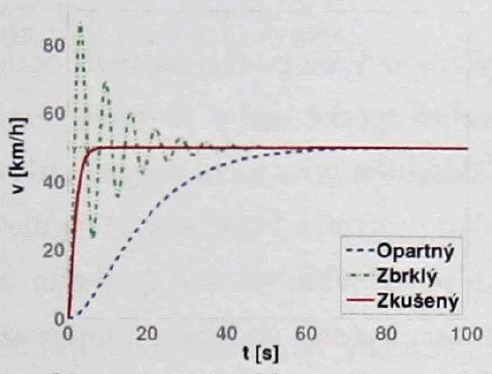
\includegraphics[width=0.7\linewidth]{Reg_smycka03.png}
      \caption{Rychlost automobilu \cite[s.~9]{Roubal2011}.}
      \label{tky:fig_feedback005}
    \end{figure}
    Pro kvalitní dosažení žádané hodnoty rychlosti je třeba znát \emph{dynamický model} automobilu. 
    Tedy nejen sešlápni pedál plynu, uvolni pedál plynu, což můžeme považovat za \emph{statický 
    model} (v čase neproměnný), ale právě popis jak rychle se automobil rozjíždí, když takovým a 
    takovým způsobem sešlápneme pedál plynu. V regulační technice budeme mít dynamický model 
    systému tvořený převážně diferenciálními (pohybovými) rovnicemi. Modelováním reálných 
    dynamických systémů se budeme zabývat v kapitole \ref{TKY:sec002}. Procesu získávání modelu 
    fyzikální reality říkáme \textbf{identifikace systému} a v našem příkladě s automobilem ji 
    vlastně provádíme tím, že se učíme jezdit. Na identifikaci dynamických systémů a její praktické 
    aspekty se zaměříme v kapitole \ref{TKY:sec003}.

    V momentě, kdy máme dynamický model systému, přichází další krok a to je vlastní \textbf{návrh 
    regulátoru}, neboli návrh algoritmu řízení. V momentě, kdy už řidič ví, jak automobil reaguje 
    na změny vstupu, může dosáhnout žádané výstupní veličiny mnohem lépe, viz obr. 
    \ref{tky:fig_feedback003}. Na rozdíl od řidiče, jenž má naučený regulátor ve své hlavě, v 
    regulační technice budeme využívat různé matematické metody. Možná nás nyní napadne, že model 
    automobilu není pouze závislost mezi pedálem plynu a rychlostí automobilu. Chování automobilu 
    ovlivňuje samozřejmě mnoho dalších okolností, jako je přilnavost pneumatik k povrchu vozovky, 
    vlhkost vozovky a podobně. V momentě, kdy například zaprší, může řidič se svým regulátorem v 
    zatáčce opustit vozovku, pokud jsme příliš agresivní, protože se reálný systém změnil, ale jeho 
    model tuto informaci nemá. Opět tedy musíme vzít v potaz nové faktory a provést identifikaci 
    znovu, a tím získat více informací o chování systému za těchto podmínek. Pak bude řidič schopen 
    jezdit bezpečně za sucha i za mokra a tak dále. V regulační technice je vždy přesnost modelu 
    zásadní otázkou. Na jedné straně požadujeme model systému co nejpřesnější, abychom byli schopni 
    navrhnout dobrý regulátor. Na druhé straně se pro příliš složitý model navrhuje regulátor 
    obtížněji. Proto vždy musíme zvolit jistý kompromis tak, aby v modelu byly zahrnuty všechny 
    podstatné vlastnosti systému.

    Tím ale regulace nekončí. Například cena paliva není již dnes zanedbatelná, a tak budeme třeba 
    chtít jezdit s minimální spotřebou. To znamená, že musíme zjistit závislost spotřeby paliva na 
    stylu jízdy. Poté musíme definovat nějaké kritérium kvality regulace obsahující tuto závislost 
    a podle něho navrhnout nový regulátor, který zajistí minimální spotřebu paliva.  Problémů v 
    oblasti řízení je samozřejmě mnohem a mnohem víc  (odhadování a filtrace, robustní řízení a 
    nelineární systémy). My však zde tento příklad ukončíme s konstatováním, že v regulační 
    technice jde především o tyto body:
    \begin{itemize}\addtolength{\itemsep}{-0.5\baselineskip}
      \item určení vstupů a výstupů systému,
      \item identifikace systému (určení chování systému na výstupech pro nějaké chování vstupů),
      \item návrh regulátoru pro zajištění požadovaných vlastností; testování regulátoru na 
            počítači; aplikace regulátoru na reálném systému; případně návrh v nějakém smyslu 
            optimálního regulátoru.
    \end{itemize}
    
  \section{Regulační smyčka a základní typy PID regulátorů}\label{TKY:sec001}
    Ve snaze řídit systémy rozeznáváme dva hlavní způsoby řízení:
      \begin{itemize}
        \item \textbf{přímovazební},
        \item \textbf{zpětnovazební}.
      \end{itemize}
    \textbf{Přímovazební řízení} (\emph{řízení v otevřené smyčce}), zvané také jako ovládání, má 
    jednodušší zapojení, ovšem jeho nevýhodou je nemožnost reagovat na poruchy či změny soustavy a 
    my se jím zde dále zabývat nebudeme. Naproti tomu \textbf{zpětnovazební řízení} (\emph{řízení v 
    uzavřené smyčce}), obecně označované jako \textbf{regulace}, porovnává \emph{výstup soustavy} 
    \(y(t)\) s \emph{požadovaným výstupem} \(w(t)\), a podle této informace generuje \emph{akční 
    zásah} \(u(t)\) do řízeného systému. Regulace nám tak dává mimo jiné možnost 
    \emph{stabilizovat} nestabilní soustavy.

    \begin{figure}[ht!] % \ref{tky:fig_feedback003}
      \centering
      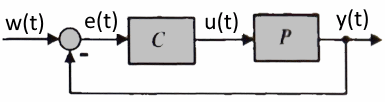
\includegraphics[width=0.8\linewidth]{Reg_smycka01.png}
      \caption{Regulační smyčka \cite[s.~215]{Roubal2011}.}
      \label{tky:fig_feedback003}
    \end{figure}
    V této kapitole se budeme věnovat regulaci, regulační smyčce a základním typů regulátorů. 
    Ukážeme si dvě základní zapojení regulačních smyček a zavedeme jednotné názvosloví, zejména 
    proto, že toto názvosloví není ustálené. Vysvětlíme si některé míry kvality řízení a ukážeme 
    názorně na příkladech vlastnosti základních \textbf{PID regulátorů}. Zvláštní pozornost bude 
    věnována filtraci derivační složky u tohoto regulátoru. Konkrétní způsoby návrhu regulátorů si 
    ukážeme v následujících kapitolách.
    
  
  \section{Modelování fyzikálních systémů}\label{TKY:sec002}
    Doposud jsme se v předešlých kapitolách zabývali různými nástroji, jak popisovat dynamické 
    chování systémů. Šlo spíše o teorii rozdělenou do kapitol bez větších souvislostí. V této kar 
    kapitole bychom chtěli ukázat použití těchto teoretických poznatků na konkrétních příkladech 
    fyzikálních systémů. Odvodíme zde několik matematických modelů fyzikálních systémů a připravíme 
    k těmto modelům simulinkové soubory s virtuální realitou pro Matlab (The Mathworks, 2009).
    
  \section{Identifikace systémů}\label{TKY:sec003}
    
%---------------------------------------------------------------------------------------------------
\printbibliography[title={Seznam literatury}, heading=subbibliography]
\addcontentsline{toc}{section}{Seznam literatury} 
%========================= Kapitola: Měření teploty ================================================
  % !TeX spellcheck = cs_CZ
%===============Kapitola: Měření teploty ===========================================================
\sisetup{
output-decimal-marker = {,},
}

\chapter{Snímače tepelných veličin}
\minitoc

  \section{Základní pojmy}
    \href{http://cs.wikipedia.org/wiki/Teplota}{Teplota} je charakteristika tepelného stavu hmoty.
    V obecném významu je to vlastnost předmětů a okolí, kterou je člověk schopen vnímat a přiřadit
    jí pocity studeného, teplého či horkého. V přírodních a technických vědách a jejich aplikacích
    je to \emph{skalární intenzivní veličina}, která je vzhledem ke svému pravděpodobnostnímu
    charakteru vhodná k popisu stavu ustálených makroskopických systémů. Teplota souvisí s
    kinetickou energií částic látky.

    Teplota je základní fyzikální veličinou soustavy \texttt{SI} s jednotkou kelvin (\si{\kelvin})
    a vedlejší jednotkou stupeň Celsia (\si{\degreeCelsius}). Nejnižší možnou teplotou je teplota
    absolutní nuly (\SI{0}{\kelvin}, resp. \SI{-273.15}{\degreeCelsius}), ke které se lze 
    libovolně
    přiblížit, avšak nelze jí dosáhnout.
         
    Do této skupiny patří především rozsáhlá část snímačů teploty. Z hlediska měřených veličin
    můžeme provést následující rozdělení.
    \begin{enumerate}\addtolength{\itemsep}{-0.5\baselineskip}
      \item \textbf{Snímače teploty}
        \begin{enumerate}[label=\emph{\alph*})]
          \item emph{Snímače pro dotykové měření} 
            \begin{itemize}
              \item elektrické
               \begin{itemize}
                 \item odporové kovové
                 \item odporové polovodičové
                 \item termoelektrické
                 \item polovodičové 
               \end{itemize}   
              \item dilatační
              \item termoelektrické
              \item tlakové
              \item speciální
            \end{itemize}
          \item \emph{Snímače pro bezdotykové měření}
            \begin{itemize}
              \item monochromatické pyrometry
              \item pásmové pyrometry
              \item radiační pyrometry
            \end{itemize}
        \end{enumerate}
      \item \textbf{Snímače tepla}
      \item \textbf{Snímače tepelného toku}
    \end{enumerate}  
       
      \subsection{Elektrické teploměry}
        \subsection{Odporové snímače}
          Odporové snímače využívají princip změny elektrického opdoru vlivem změny teplot.
          Základním požadavkem kladeným na materiál snímače je co největší a stálý teplontí
          součinitel odporu a zároveň co největší měrný odpor. Pro tyto účely se používají kovové a
          polovodičové materiály.
          
          \subsubsection{Kovové odporové snímače} 
            Jsou to především čisté kovy, které se používají pro realizaci vlastního odporového
            článku. Požadavkem je, aby nereagovaly s izolačním nebo ochranným krytem. Jakékoliv
            chemické nebo fyzikální vlivy by mohly způsobit nestálost odporu při stálé teplotě,
            Použitý materiál nemá vykazovat změnu teplotního součinitele odporu s časem (stárnutí)
            a hysterezi. Nejčastěji používanými materiály je \emph{platina, nikl, měď, slitina
            stříbro-zlato} a další \cite[s.~96]{Zehnula1983}.
             
            Platina je výhodná pro velkou chemickou stálost, vysokou teplotou tavení a možností
            dosažení vysoké čistoty. Pro snímače teploty se používá tzv. fyzikálně  čistá platina,
            jejíž čistota se pohybuje kolem 99,93 až 99,99 \% Pt. Měření ukázala, že změny
            základního odporu u sériově vyráběných přesných teploměru se pohybí kolem
            \num{5e-6}$R_o$ (což odpovídá \SI{0.001}{\kelvin}), u nejlepších teploměrů je tato
            hodnota ještě o řád menší. Proto se používá platina pro etalonový teplměr v oblasti
            teplot \SI{-259.34}{\degreeCelsius} až \SI{630.74}{\degreeCelsius}.
            
            Závislost odporu na teplotě pro rozsah \num{0} až \SI{630}{\degreeCelsius} se vyjadřuje
            rovnicí
            \begin{equation}\label{SAC:kov_Ro1}
              R_\vartheta = R_0(1 + A\vartheta + B\vartheta^2)
            \end{equation}
            kde 
            \begin{labeling}{$\omega t+\varphi_0$}
              \setlength{\itemindent}{2cm}
              \item[\(R_0\)]          \(\ldots\) \emph{odpor při \SI{0}{\degreeCelsius}}, 
              \item[\(\vartheta\)]    \(\ldots\) \emph{teplota ve \si{\degreeCelsius}}, 
              \item[\(A\)]            \(\ldots\) \emph{konst (\SI{3.9075e-3}{\per\degreeCelsius})},
              \item[\(B\)]            \(\ldots\) \emph{konst (\SI{-0.575e-6}{\per\degreeCelsius})}. 
            \end{labeling}
 
             V rozmezí od \SI{0}{\degreeCelsius} do \SI{-190}{\degreeCelsius} se vyjadřuje
             závislost odporu na teplotě rovnicí
             \begin{equation}\label{SAC:kov_Ro2}
               R_\vartheta = R_0[1 + A\vartheta + B\vartheta^2 + C(\vartheta - 100)\vartheta^3)]
             \end{equation}

%---------------------------------------------------------------------------------------------------
\printbibliography[title={Seznam literatury}, heading=subbibliography]
\addcontentsline{toc}{section}{Seznam literatury}
  
}